\documentclass[11pt, a4paper]{article}

% Language setting
% Replace `english' with e.g. `spanish' to change the document language
\usepackage[italian]{babel}

% Set page size and margins
% Replace `letterpaper' with`a4paper' for UK/EU standard size
\usepackage[a4paper,top=2cm,bottom=2cm,left=3cm,right=3cm,marginparwidth=1.75cm]{geometry}

% Useful packages
\usepackage{float}
\usepackage{amsmath}
%\usepackage{graphicx}
%\usepackage[colorlinks=true, allcolors=black]{hyperref}
%\usepackage{makeidx}
\usepackage{algorithm}
\usepackage{algorithmicx}
\usepackage{algpseudocode}
\usepackage{mathtools}
\usepackage{varwidth}
\usepackage{tikz}
\usepackage{subcaption}

\DeclareRobustCommand{\willy}[1]{
\definecolor{mycolor#1}{RGB}{#1,#1,#1}
}
\willy{0}
\willy{1}
\willy{2}
\willy{3}
\willy{4}
\willy{5}
\willy{6}
\willy{7}
\willy{8}
\willy{9}
\willy{10}
\willy{11}
\willy{12}
\willy{13}
\willy{14}
\willy{15}
\willy{16}
\willy{17}
\willy{18}
\willy{19}
\willy{20}
\willy{21}
\willy{22}
\willy{23}
\willy{24}
\willy{25}
\willy{26}
\willy{27}
\willy{28}
\willy{29}
\willy{30}
\willy{31}
\willy{32}
\willy{33}
\willy{34}
\willy{35}
\willy{36}
\willy{37}
\willy{38}
\willy{39}
\willy{40}
\willy{41}
\willy{42}
\willy{43}
\willy{44}
\willy{45}
\willy{46}
\willy{47}
\willy{48}
\willy{49}
\willy{50}
\willy{51}
\willy{52}
\willy{53}
\willy{54}
\willy{55}
\willy{56}
\willy{57}
\willy{58}
\willy{59}
\willy{60}
\willy{61}
\willy{62}
\willy{63}
\willy{64}
\willy{65}
\willy{66}
\willy{67}
\willy{68}
\willy{69}
\willy{70}
\willy{71}
\willy{72}
\willy{73}
\willy{74}
\willy{75}
\willy{76}
\willy{77}
\willy{78}
\willy{79}
\willy{80}
\willy{81}
\willy{82}
\willy{83}
\willy{84}
\willy{85}
\willy{86}
\willy{87}
\willy{88}
\willy{89}
\willy{90}
\willy{91}
\willy{92}
\willy{93}
\willy{94}
\willy{95}
\willy{96}
\willy{97}
\willy{98}
\willy{99}
\willy{100}
\willy{101}
\willy{102}
\willy{103}
\willy{104}
\willy{105}
\willy{106}
\willy{107}
\willy{108}
\willy{109}
\willy{110}
\willy{111}
\willy{112}
\willy{113}
\willy{114}
\willy{115}
\willy{116}
\willy{117}
\willy{118}
\willy{119}
\willy{120}
\willy{121}
\willy{122}
\willy{123}
\willy{124}
\willy{125}
\willy{126}
\willy{127}
\willy{128}
\willy{129}
\willy{130}
\willy{131}
\willy{132}
\willy{133}
\willy{134}
\willy{135}
\willy{136}
\willy{137}
\willy{138}
\willy{139}
\willy{140}
\willy{141}
\willy{142}
\willy{143}
\willy{144}
\willy{145}
\willy{146}
\willy{147}
\willy{148}
\willy{149}
\willy{150}
\willy{151}
\willy{152}
\willy{153}
\willy{154}
\willy{155}
\willy{156}
\willy{157}
\willy{158}
\willy{159}
\willy{160}
\willy{161}
\willy{162}
\willy{163}
\willy{164}
\willy{165}
\willy{166}
\willy{167}
\willy{168}
\willy{169}
\willy{170}
\willy{171}
\willy{172}
\willy{173}
\willy{174}
\willy{175}
\willy{176}
\willy{177}
\willy{178}
\willy{179}
\willy{180}
\willy{181}
\willy{182}
\willy{183}
\willy{184}
\willy{185}
\willy{186}
\willy{187}
\willy{188}
\willy{189}
\willy{190}
\willy{191}
\willy{192}
\willy{193}
\willy{194}
\willy{195}
\willy{196}
\willy{197}
\willy{198}
\willy{199}
\willy{200}
\willy{201}
\willy{202}
\willy{203}
\willy{204}
\willy{205}
\willy{206}
\willy{207}
\willy{208}
\willy{209}
\willy{210}
\willy{211}
\willy{212}
\willy{213}
\willy{214}
\willy{215}
\willy{216}
\willy{217}
\willy{218}
\willy{219}
\willy{220}
\willy{221}
\willy{222}
\willy{223}
\willy{224}
\willy{225}
\willy{226}
\willy{227}
\willy{228}
\willy{229}
\willy{230}
\willy{231}
\willy{232}
\willy{233}
\willy{234}
\willy{235}
\willy{236}
\willy{237}
\willy{238}
\willy{239}
\willy{240}
\willy{241}
\willy{242}
\willy{243}
\willy{244}
\willy{245}
\willy{246}
\willy{247}
\willy{248}
\willy{249}
\willy{250}
\willy{251}
\willy{252}
\willy{253}
\willy{254}
\willy{255}

\usetikzlibrary{automata, positioning, decorations.text, topaths, arrows.meta, decorations.pathmorphing, quotes, shapes.geometric, arrows}
\DeclarePairedDelimiter\floor{\lfloor}{\rfloor}

\tikzset{
->, % makes the edges directed
%>=stealth’, % makes the arrow heads bold
node distance=1cm, % specifies the minimum distance between two nodes. Change if necessary.
every state/.style={thick, fill=gray!10}, % sets the properties for each ’state’ node
initial text=$ $, % sets the text that appears on the start arrow
}

%for code
\usepackage{listings}

\makeatletter
\long\def\@makecaption#1#2{%
  \vskip\abovecaptionskip
    \bfseries #1: #2\par
  \vskip\belowcaptionskip}%
\makeatother

%\usepackage{color}

%\definecolor{dkgreen}{rgb}{0,0.6,0}
%\definecolor{gray}{rgb}{0.5,0.5,0.5}
%\definecolor{mauve}{rgb}{0.58,0,0.82}


\lstset{frame=tb,
  language=VHDL,
  aboveskip=3mm,
  belowskip=3mm,
  showstringspaces=false,
  columns=flexible,
  basicstyle={\small\ttfamily},
  numbers=left,
  numberstyle=\tiny\color{gray},
  keywordstyle=\color{blue},
  commentstyle=\color{dkgreen},
  stringstyle=\color{mauve},
  breaklines=true,
  breakatwhitespace=true,
  tabsize=3,
  backgroundcolor=\color{white}
}

\title{Progetto di Reti Logiche}
\author{
  William Zeni\\
  \texttt{matricola 10613915}
  \and
  Cristina Urso\\
  \texttt{matricola 10599689}
}

\date{Anno 2020/21}

\graphicspath{ {./graphics/} }

\makeindex

\begin{document}

\begin{figure}[t]
  \centering
  \vspace{3cm}
  
\includegraphics[scale=0.4]{Logo_Politecnico_Milano.png}
  \vspace{3cm}
\end{figure}

\maketitle
\renewcommand{\abstractname}{ }
\begin{abstract}
  \centering
  Progetto sostenuto presso il Politecnico di Milano - Dipartimento di Elettronica, Informazione e Bioingegneria. Corso diretto dal Prof. Gianluca Palermo.
\end{abstract}

\thispagestyle{empty}
\pagebreak
\tableofcontents
\thispagestyle{empty}
\pagebreak
\pagenumbering{arabic}


\section{Introduzione}
\subsection{Scopo del progetto}
Lo scopo del progetto è quello di creare un componente hardware sintetizzabile, in grado di equalizzare un immagine. L'algoritmo che ne prevede l'equalizzazione si ispira ad una versione semplificata del metodo di equalizzazione dell'istogramma, il quale applica un aumento nel contrasto di un immagine su scala di grigi. In generale l'elaborazione digitale dell'immagine risulta più evidente specialmente quando i dati raccolti sono rappresentati da valori di intensità molto vicini. Per cui, se una immagine contenesse una scala di grigi molto ampia, l'effeto dell'equalizzazione risulterebbe pressochè nullo.

\subsection{Specifiche generali}
Si definisca un immagine dalle dimensioni variabili, ma di massimo $128 \times 128$, e si definisca una memoria lineare nella quale i primi due valori siano le dimensioni dell'immagine e i restanti i valori assegnati ad ogni pixel, il componente hardware dovrà scrivere in coda alla memoria l'immagine equalizzata pixel per pixel.
Il risultato sarà una memoria complessivamente lunga $2 \cdot N_{col} \cdot N_{row} +2$, dove $N_{row}$ e $N_{col}$ sono rispettivamente il numero di righe e di colonne dell'immagine. A partire dalla posizione 2, per ogni pixel si avrà il corrispettivo pixel equalizzato ad una distanza $N_{col} \cdot N_{row}$ come mostrato in figura.
\\
\\

\begin{tikzpicture}
\draw[step=1cm, black,very thin] (0,0) grid (13,1);
\fill[text=black] (0.5,0.5) node{$N_{col}$};
\fill[text=black] (0.5,1.3) node{$0$};
\fill[text=black] (1.5,0.5) node{$N_{row}$};
\fill[text=black] (1.5,1.3) node{$1$};
\fill[blue!30!white, draw=black] (2,0) rectangle (3,1);
\fill[text=black] (2.5,1.3) node{$2$};
\fill[green!30!white, draw=black] (3,0) rectangle (4,1);
\fill[text=black] (3.5,1.3) node{$3$};
\fill[red!30!white, draw=black] (4,0) rectangle (5,1);
\fill[text=black] (4.5,1.3) node{$4$};
\fill[text=black] (5.5,0.5) node{\dots};
\fill[text=black] (6.5,0.5) node{\dots};
\fill[text=black] (7.5,0.5) node{\dots};
\fill[blue!30!white, draw=black] (8,0) rectangle (9,1);
\fill[text=black] (8.5,1.3) node{$N_{col}\cdot N_{row}+2$};
\fill[text=black] (8.5,-0.5) node{\texttt{new\_pixel}};
\fill[green!30!white, draw=black] (9,0) rectangle (10,1);
\fill[red!30!white, draw=black] (10,0) rectangle (11,1);
\fill[text=black] (11.5,0.5) node{\dots};
\end{tikzpicture}
\\
La memoria dialogherà in stretto contatto con il componente attraverso due segnali, che determineranno l'avvio della computazione, la sua terminazione e l'eventuale ripartenza. Si noti che la computazione di una singola immagine, una volta iniziata, non potrà mai essere interrotta, ma rimane possibile la computazione di più immagini.\\
\\
Ogni pixel avrà un valore compreso tra $0$ e $255$ e verrà rielaborato dal componente nel seguente modo:\\
\\

\noindent\fbox{
\begin{varwidth}{\dimexpr\linewidth-2\fboxsep-2\fboxrule\relax}

\begin{algorithmic}[1]
  \State $delta\_value \gets max\_pixel\_value - min\_pixel\_value$
  \State $shift\_level \gets 8 - \floor{\log_2(delta\_value+1)}$
  \State $temp\_pixel \gets curr\_pixel\_value - min\_pixel\_value$
  \State $temp\_pixel \gets temp\_pixel << shift\_level$
  \If{$temp\_pixel > 255$}
    \State $new\_pixel \gets 255$
  \Else
    \State $new\_pixel \gets temp\_pixel$
  \EndIf
\end{algorithmic}

\end{varwidth}
}
\\
\\
\\
dove \texttt{max\_pixel\_value} e \texttt{min\_pixel\_value} sono rispettivamente il valore massimo e il valore minimo del pixel trovati all'interno dell'immagine, \texttt{curr\_pixel\_value} è il valore del pixel preso in considerazione e \texttt{new\_pixel} è il valore del pixel da scrivere in memoria.
\pagebreak

\subsection{Interfaccia del componente}
\begin{lstlisting}
entity project_reti_logiche is
port (
    i_clk       : in std_logic;
    i_rst       : in std_logic;
    i_start     : in std_logic;
    i_data      : in std_logic_vector(7 downto 0);
    o_address   : out std_logic_vector(15 downto 0);
    o_done      : out std_logic;
    o_en        : out std_logic;
    o_we        : out std_logic;
    o_data      : out std_logic_vector (7 downto 0)
);
end project_reti_logiche;
\end{lstlisting}
L'interfaccia del componente, per potersi relazionare con la memoria, deve essere come quella sopra riportata. I segnali di input vengono evidenziati dal prefisso \texttt{\lq i\_'}, mentre per i segnali di output è presente il prefisso \texttt{\lq o\_'}. Nel dettaglio:
\begin{itemize}
  \item \textbf{i\_clk} scandisce il ciclo di clock della memoria, registrando \lq$1$' sul \texttt{rising\_edge}.
  \item \textbf{i\_rst} è il segnale di \texttt{RESET}, viene chiamato all'inizio della computazione di una o più immagini. Se si registra \lq$1$' su questo segnale la computazione deve essere terminata e ripristinata al momento di partenza.
  \item \textbf{i\_start} determina l'inizio della coputazione. Questo segnale rimane alto fino a quando la computazione non termina. La computazione può iniziare solo se il segnale è basso.
  \item \textbf{i\_data} raccoglie i dati inviati dalla memoria.
  \item \textbf{o\_address} è il segnale attraverso il quale si possono fare richieste alla memoria. Sostanzialmente su questo segnale si pone l'indirizzo della memoria che si vuuole leggere o sulla quale si vuole scrivere.
  \item \textbf{o\_done} determina la fine della computazione. Il segnale deve essere portato alto quando si vuole terminare la computazione e deve rimanere alto fino a quando la memoria non porti il segnale di \texttt{START} basso. Solo in quel caso il segnale viene riportato basso.
  \item \textbf{o\_en} abilita la memoria alla lettura o alla scrittura.
  \item \textbf{o\_we}  abilita la memoria alla scrittura. Quando questo segnale è alto la memoria si aspetta un dato in ingresso da scrivere.
  \item \textbf{o\_data} è il dato che la memoria si aspetta di leggere quando la scrittura è attiva.
\end{itemize}
\pagebreak
\subsection{Dati e Descrizione memoria}
\begin{lstlisting}[title={Fig.1}]
architecture projecttb of project_tb is
  constant    c_CLOCK_PERIOD     : time := 15 ns;
  signal      mem_address        : std_logic_vector (15 downto 0);
  signal      mem_o_data         : std_logic_vector (7 downto 0);
  signal      mem_i_data         : std_logic_vector (7 downto 0);
  signal      tb_done            : std_logic;
  signal      tb_rst             : std_logic;
  signal      tb_start           : std_logic;
  signal      tb_clk             : std_logic;
  signal      enable_wire        : std_logic;
  signal      mem_we             : std_logic;

type ram_type is array (65535 downto 0) of std_logic_vector(7 downto 0);
\end{lstlisting}
\begin{lstlisting}[title={Fig. 2}]
begin
UUT: project_reti_logiche
port map (
          i_clk       => tb_clk,
          i_start     => tb_start,
          i_rst       => tb_rst,
          i_data      => mem_o_data,
          o_address   => mem_address,
          o_done      => tb_done,
          o_en        => enable_wire,
          o_we        => mem_we,
          o_data      => mem_i_data
          );
\end{lstlisting}
La memoria ha un'interfaccia che dialoga direttamente con il componente sintetizzato come indicato dalla \textit{port map} rappresentata in \texttt{Fig.2}. È indirizzabile al \textit{byte} e ha una dimensione massima di $N_{col}*N_{row}*2+2$ dove nel caso pessimo $N_{col}$ e $N_{row}$ hanno un valore di $128$ \textit{byte}. Pertanto, la dimensione massima supportabile dalla memoria deve essere di $2^7 * 2^7 *2 + 2$, ovvero di $32770$ \textit{byte}. Come si può notare dalla definizione della sua entity (\texttt{Fig.1}), per evitare eventuali errori, si è deciso di dedicare al componente uno spazio di $2^{16}$ \textit{byte}. Ogni singolo \textit{byte} è definito a sua volta da un \textit{std\_logic\_vector} di $8$ \textit{bit} di tipo \texttt{unsigned} e può avere un valore compreso tra $0$ e $255$, dove $0$ rappresenta il pixel nero e $255$ rappresenta il pixel bianco.
Qualora fosse prevista l'elaborazione di più immmagini, vi sarà la necessità di definire più memorie in cascata. \\
La costante \texttt{c\_CLOCK\_PERIOD} è quella che determina il ciclo di \textit{clock} del componente e deve essere mantenuta per specifica sotto i $100$ \textit{ns}.
\pagebreak
\section{Desing Pattern}
\subsection{Scelte Progettuali}
La struttura del progetto è stata suddivisa in due process principali: \texttt{UPDATE} e \texttt{STATES}.
Il primo ha il compito di relazionarsi con la memoria e il secondo contiene gli stati della macchina impiegati nella equalizzazione delle immagini. In questo modo una porzione di codice è adibita esclusivamente alla computazione dei pixel (process \texttt{STATES}), mentre la rimanente si occupa dei segnali di output della \textit{entity} (process \texttt{UPDATE}).\\
Per permette un corretto dialogo tra i due process è nata l'esigenza di avere dei segnali ``duplicati".
I segnali con suffisso \texttt{\lq\_cp'} sono stati introdotti per mantere in memoria i valori computati, mentre i segnali con suffisso \texttt{\lq\_next'} sono stati implementati allo scopo di permettere agli stati di far richieste alla memoria.
Nel particolare, per ogni ciclo di clock, durante il \textit{rising\_edge}, il process \texttt{UPDATE} si risveglia, aggiornando i segnali. I segnali contenenti i valori da mantenere vengono reimpostati con i segnali \texttt{\lq\_cp'}, mentre i segnali di output della \textit{entity} sono aggiornati con i segnali \texttt{\lq\_next'}.\\
Il process \texttt{STATES} è a tutti gli effetti un \texttt{FSM} (\textit{Macchina a Stati Finiti}) rappresentabile attraverso lo schema al paragrafo $2.3$.
Il suo funzionamento è permesso sostanzialmente da tre segnali a lui dedicati: \texttt{next\_state}, che identifica la chiamata allo stato prossimo,  \texttt{curr\_state}, che rileva lo stato corrente, e \texttt{prev\_state}, che conserva lo stato precedente.

\subsection{Elenco Stati - Process STATES}

\subsubsection{START}
Lo stato di \texttt{START} è il primo stato del process \texttt{STATES} ed è stato pensato come stato di attesa iniziale. Questo stato viene invocato in due situazioni differenti: se il segnale di \texttt{i\_rst} viene portato alto, oppure quando il segnale \texttt{i\_start} viene riportato basso dopo la computazione di un immagine. Lo stato \texttt{START} non cambia fino a quando il segnale \texttt{i\_start} non viene portato alto. In quel momento lo stato successivo viene impostato a \texttt{INIT}.

\subsubsection{INIT}
\texttt{INIT} è uno stato di transizione nel quale il processore si assicura che i segnali siano inizializzati con i valori opportuni. Successivamente imposta lo stato prossimo a \texttt{ABILIT\_READ}.

\subsubsection{ABILIT\_READ}
Attraverso \texttt{ABILIT\_READ} si abilita la memoria alla sola lettura. Viene richiamato in due momenti diversi del progetto: all'inizio della computazione, subito dopo \texttt{INIT}, per portare il segnale \texttt{o\_en} a $1$ e permettere agli altri stati di poter leggere dalla memoria, oppure dopo la scrittura di un pixel, al fine di disabilitare l'accesso alla scrittura. In base allo stato chiamante, instrada lo stato prossimo a quello opportuno.

\subsubsection{ABILIT\_WRITE}
Lo stato \texttt{ABILIT\_WRITE} abilita la memoria alla scrittura. Viene invocato subito dopo aver computato il valore del nuovo pixel e in nessun altro momento. Instrada poi lo stato prossimo a \texttt{WRITE\_PIXEL}.

\pagebreak
\subsubsection{WAIT\_MEM}
\texttt{WAIT\_MEM} è uno stato centrale durante la gestione del flusso di dati. La sua funzione è quella di far ``sprecare" un ciclo di clock al processore. Ciò ci assicura sia in caso di scrittura, sia in caso di lettura, che i segnali in ingresso e in uscita siano letti o scritti correttamente. Nello specifico, questo stato evita che lo stato successivo lavori con dati relativi allo stato precedente. In base allo stato chiamante instrada lo stato prossimo in modo opportuno.\\ \\
\textbf{N.B:} \textit{Alcune chiamate a questo stato potevano essere evitate. Questa informazione è emersa durante lo stress test a cui il processore è stato sottoposto. Tuttavia, è stato scelto di forzare ugualmente l’attesa per ovviare eventuali errori e per permettere la corretta acquisizione dei dati indipendentemente dal periodo di clock scelto. Ciò dovrebbe permettere una maggior robustezza, sebbene un aumento nella latenza della computazione.}

\subsubsection{GET\_RC}
\texttt{GET\_RC} si occupa della lettura dei primi due pixel della memoria in cui sono contenute le dimensioni dell’immagine da modificare. Viene invocato dopo l'abilitazione della memoria alla lettura e aggiorna i segnali \texttt{n\_col} e \texttt{n\_row}. Lo stato richiama se stesso fino a quando non ha aggiornato i due segnali, altrimenti imposta lo stato prossimo a \texttt{GET\_DIM}.

\subsubsection{GET\_DIM}
Lo stato \texttt{GET\_DIM} si preoccupa di aggiornare il segnale \texttt{dim\_address} con l'indirizzo del primo \textit{byte} libero per la scrittura. Il calcolo che ne determina il valore è: $n\_col \cdot n\_row + 2$.\\
\texttt{GET\_DIM} verifica inoltre il caso speciale in cui una delle dimensioni dovesse essere nulla. In quel caso impone lo stato prossimo a \texttt{DONE}.\\ \\
\textbf{N.B:}\textit{
La moltiplicazione usa segnali \textit{std\_logic\_vector} da $8$ bit e produce un risultato su $16$ bit. Essendo \texttt{dim\_address} un \textit{std\_logic\_vector} su $16$ bit, il problema non si pone.
}

\subsubsection{READ\_PIXEL}
\texttt{READ\_PIXEL} è uno stato strettamente connesso con lo stato \texttt{GET\_MINMAX}. Richiede alla memoria il valore del pixel da leggere e aggiorna il segnale \texttt{curr\_address} a quello successivo. In questo modo il valore del pixel sarà disponibile sul segnale \texttt{i\_data} dopo due \textit{rising\_edge}. L'attesa è sempre lasciata allo stato \texttt{WAIT\_MEM}.

\subsubsection{GET\_MINMAX}
\texttt{GET\_MINMAX} aggiorna i segnali \texttt{max\_pixel\_value} e \texttt{min\_pixel\_value}, inizializzati rispettivamente con $0$ e $255$, con il valore di \texttt{i\_data}. Questo avviene se e solo se si verifica che \texttt{i\_data} è \textit{maggiore} di \texttt{max\_pixel\_value} (in questo caso aggiorna \texttt{max\_pixel\_value}) oppure se \texttt{i\_data} è \textit{minore} di \texttt{min\_pixel\_value} (in questo caso aggiorna \texttt{min\_pixel\_value}). Infine, imposta lo stato prossimo a \texttt{READ\_PIXEL}
%non so perche lo mette in viola

\subsubsection{GET\_DELTA}
\texttt{GET\_DELTA} è uno stato banale. Calcola la \textit{differenza} tra \texttt{max\_pixel\_value} e \texttt{min\_pixel\_value} e imposta lo stato prossimo a \texttt{WAIT\_MEM}.

\pagebreak

\subsubsection{CALC\_SHIFT}
Lo stato \texttt{CALC\_SHIFT} si preoccupa di effettuare la riga $2$ dello speudo-codice riportato al paragrafo $1.2$.
Per effettuare il calcolo, richiama se stesso (attraverso lo stato \texttt{WAIT\_MEM}) aggiornando dei segnali d'appoggio. Nel dettaglio si potrebbe semplificare il tutto con il seguente pseudo-codice:
\\
\\
\noindent\fbox{
\begin{varwidth}{\dimexpr\linewidth-2\fboxsep-2\fboxrule\relax}
\begin{algorithmic}[1]
  \State $m \gets delta\_value+1$
  \State $k \gets -1$
  \State $t \gets 1$
   \While{$t\leq m$}
   \State $k \gets k+1$
       \State $t \gets t*2$
  \EndWhile
  \State $shift\_level \gets 8-k$
\end{algorithmic}
\end{varwidth}
}
\\
\\
\\
Sostanzialmente attraverso il ciclo \texttt{WHILE} si ricava \textit{k}, il quale non è altro che il valore di $\floor{log_2(delta\_value +1)}$. Questa procedura è forse quella più dispendiosa a livello di tempo e memoria, poichè per aggiornare ogni segnale si deve come minimo attendere due cicli di clock. Inoltre, la moltiplicazione tra due interi (\textit{t} e $2$) produce un risultato su $64$ \textit{bit} che VHDL gestisce troncando a $32$ \textit{bit}. Per le specifiche del progetto, ci si aspetta che \textit{k} non possa assumere un valore maggiore di $8$. Pertanto, si è certi che una variabile a $32$ \textit{bit} possa largamente contenere i valori desiderati.

\subsubsection{GET\_PIXEL}
\texttt{GET\_PIXEL} è uno stato omonimo di \texttt{READ\_PIXEL}. La principale differenza del primo con il secondo è che mentre \texttt{READ\_PIXEL} effettua dei controlli sul flusso della computazione, \texttt{GET\_PIXEL} richiede solamente alla memoria il dato da leggere e imposta lo stato prossimo a \texttt{WAIT\_MEM}.

\subsubsection{CALC\_NEWPIXEL}
In \texttt{CALC\_NEWPIXEL} si calcola il nuovo valore del pixel da scrive in memoria.
Per farlo, viene utilizzata una variabile di appoggio \texttt{pixel\_to\_shift} definita come uno \textit{std\_logic\_vector} da $16$ \textit{bit} e inizializzata come $\texttt{i\_data}-\texttt{min\_pixel\_value}$ con l’aggiunta di otto `$0$' in posizione più significativa.
La variabile viene, quindi, shiftata e su di essa viene fatto il seguente controllo: se risulta essere minore di $255$ allora aggiorniamo il segnale \texttt{new\_pixel} al suo valore in \textit{std\_logic\_vector} su $8$ \textit{bit}, altrimenti il segnale \texttt{new\_pixel} viene impostato a $255$ sempre in \textit{std\_logic\_vector} su $8$ \textit{bit}.

\subsubsection{WRITE\_PIXEL}
Lo stato \texttt{WRITE\_PIXEL} si assicura che il valore del nuovo pixel calcolato sia scritto in memoria, incrementa tutti i contatori e controlla di non essere arrivato al termine della computazione. Il controllo usufruisce della varibile intera \texttt{last}, che assume il valore di $2*\texttt{n\_col}*\texttt{n\_row}+2$, ovvero l'indice dell'ultimo pixel scrivibile. Quando il contatore assume questo valore lo stato successivo viene impostato a \texttt{DONE} (sempre attravero \texttt{WAIT\_MEM}), altrimenti viene impostato lo stato prossimo a \texttt{ABILIT\_READ}, dove la scrittura viene disabilitata e viene riabilitata la lettura per il pixel successivo. Anche qui, si noti che il calcolo di \texttt{last} è sicuramente contenibile in una varibile a $32$ \textit{bit}.

\subsubsection{DONE}
\texttt{DONE} chiude tutte le comunicazioni con la memoria, riportando a `$0$' sia \texttt{o\_en} che \texttt{o\_we} e pulendo il buffer di \texttt{o\_address} e \texttt{o\_data}.
Successivamente il segnale \texttt{o\_done} viene portato ad `$1$' e lo stato prossimo è impostato a \texttt{ WAITING\_PIC}.


\subsubsection{WAITINGPIC}
Ultimo stato del processo. Ha lo scopo di restare in attesa che il segnale di \texttt{i\_start} venga riportato a `$0$'. Finche ciò non avviene, \texttt{ WAITING\_PIC} richiama se stesso. Quando sia \texttt{i\_start} che \texttt{o\_done} hanno il segnale a `$0$', imposta lo stato prossimo a \texttt{START} facendo ricominciare l’intera compilazione.

\subsection{Approfondimento sul process STATES}
All'interno del process \texttt{STATES} si possono notare due macro momenti della computazione. Il primo è quello descritto dalla prima lettura completa della memoria (da \texttt{START} a \texttt{GET\_PIXEL}), attraverso la quale si determinano tutti i valori necessari per la computazione del nuovo pixel. Si noti inoltre che all'interno del primo momento abbiamo due cicli ben distinti: uno per il calcolo del \textit{max\_value} e \textit{min\_value} e uno per il calcolo dello \textit{shift\_level}. Il secondo momento (fino a \texttt{DONE}), invece, è descritto dalla seconda lettura semi-completa della memoria (difatto si esclude la lettura dei primi $2$ \textit{byte}) ed è il momento nel quale il pixel appena letto viene rielaborato e salvato in memoria nel \textit{byte} opportuno. Questa doppia lettura della memoria, sebbene aumenti la complessità temporale, è strettamente necessaria, per via del calcolo del \textit{delta}. Iniziamente, si era pensato di ottimizzare il secondo momento con due proeccess paralleli: il primo avrebbe elaborato i pixel pari, mentre il secondo i pixel dispari, e sarebbero stati gestiti da opportuni `semafori'. Tuttavia, la struttura attuale è risultata essere molto più stabile nei test, permettendoci anche di variare a nostra discrezione il tempo di clock della computazione.
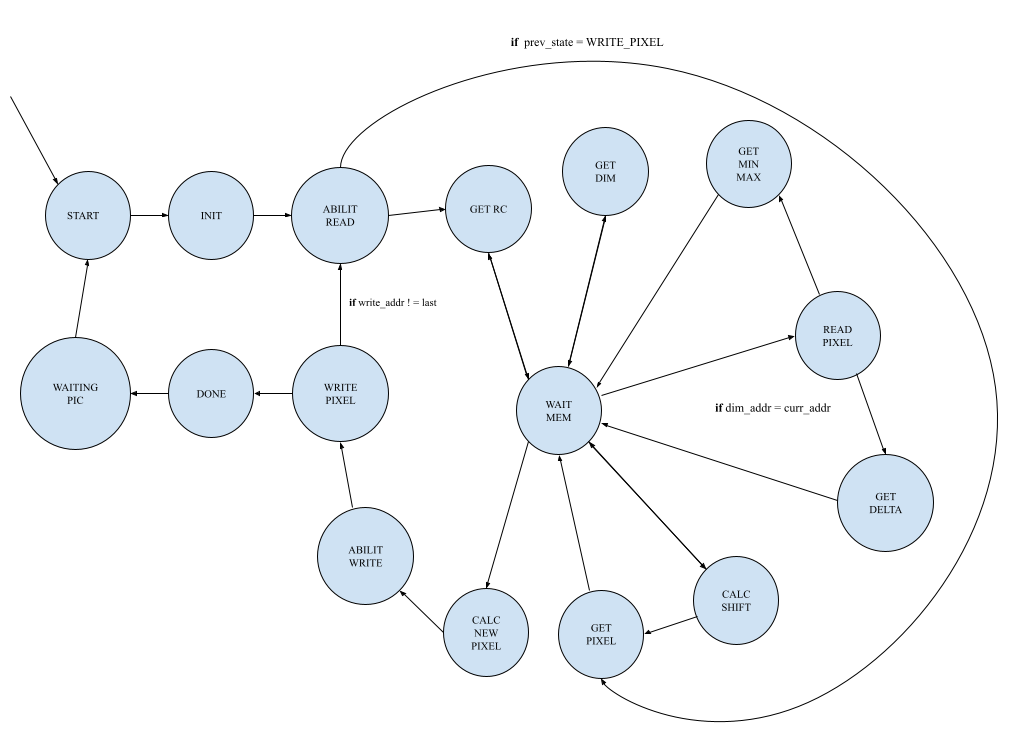
\includegraphics[width=16cm, height=11.5cm]{FSM.png}
%\pagebreak
%\subsubsection{Schema process STATES}
%FSA
%\vspace{0.5 cm}
%\begin{center}
%\resizebox{!}{24cm}{
%\begin{tikzpicture}[->,>=stealth',shorten >=1pt,auto,node distance=2cm,
%        scale = 1,transform shape, on grid]

%  \node[state] (start) [scale=1] {$START$};
%  \node[state] (init) [below=of start, scale=1]  {$INIT$};
%  \node[state] (abilitread) [below= of init, scale=0.5]  {$ABILIT\_READ$};
%  \node[state] (getrc) [below=of abilitread, scale=0.8, yshift=-0.5cm]  {$GET\_RC$};
%  \node[state] (getdim) [below=of getrc, scale=0.6]  {$GET\_DIM$};
%  \node[state] (readpixel) [below=of getdim, scale=0.5]  {$READ\_PIXEL$};
%  \node[state] (getminmax) [below =of readpixel, scale=0.5] {$GET\_MINMAX$};
%  \node[state] (getdelta) [below =of getminmax, scale=0.5] {$GET\_DELTA$};
%  \node[state] (calcshift) [below=of getdelta, scale=0.5]  {$CALC\_SHIFT$};
%  \node[state] (getpixel) [below=of calcshift, scale=0.5 ]  {$GET\_PIXEL$};
%  \node[state] (calcnewpixel) [below=of getpixel, scale=0.5]  {$CALC\_NEWPIXEL$};
%  \node[state] (abilitwrite) [below=of calcnewpixel, scale=0.5, yshift=-1cm]  {$ABILIT\_WRITE$};
%  \node[state] (writepixel) [below=of abilitwrite, scale=0.5, yshift=-1cm]  {$WRITE\_PIXEL$};
%  \node[state] (done) [below=of writepixel, scale=0.7]  {$DONE$};
%  \node[state] (waitingpic) [below=of done, scale=0.6]  {$WAITINGPIC$};
%  \node[state] (waitmem) [right=of calcshift, xshift=8cm, scale=1.2]  {$WAIT\_MEM$};

%  \draw (start) edge[red] node{} (init)
%        (init) edge[red] node{} (abilitread)
%        (abilitread) edge[red] node{} (getrc)
%        (getrc) edge[bend left, out=60, in=45, looseness=1, red] node{} (waitmem)
%        (waitmem) edge[bend right, in=-100, out=200, looseness=2, red] node{} (getrc)
%        (getdim) edge[bend left, in=120, red] node{} (waitmem)
%        (waitmem) edge[bend right, out=-70, in=-100, red] node{} (getdim)
%        (readpixel) edge[bend left, out=50, in=130, blue] node{} (waitmem)
%        (waitmem) edge[bend right, out=-30, blue] node{} (getminmax)
%        (getminmax) edge[blue] node{} (readpixel)
%        (readpixel) edge[bend right=90, red] node{} (getdelta)
%        (waitmem) edge [bend right, out=-30, red] node{} (readpixel)
%        (getdelta) edge[bend left, red] node{} (waitmem)
%        (waitmem) edge[bend right=20, brown] node{} (calcshift)
%        (calcshift) edge[bend right=20, brown] node{} (waitmem)
%        (calcshift) edge[red] node{} (getpixel)
%        (getpixel) edge[bend right, green] node{} (waitmem)
%        (waitmem) edge[bend left, out=70, green] node{} (calcnewpixel)
%        (calcnewpixel) edge[green] node{} (abilitwrite)
%        (abilitwrite) edge[green] node{} (writepixel)
%        (writepixel) edge[bend right, in=-80, green] node{} (waitmem)
%        (writepixel) edge[bend left, in=140, green] node{} (abilitread)
%        (abilitread) edge[bend right, green] node{} (getpixel)
%        (waitmem) edge[bend left, out=100, looseness=2, green] node{} (done)
%        (done) edge[green] node{} (waitingpic)
%        (waitingpic) edge[bend left] node{} (start)
%        ;
%\end{tikzpicture}
%}
%\end{center}

%\pagebreak
\section{Risultati dei Test}
I test eseguiti sono stati pensati appositamente per evitare eventuali errori di programmazione, cercando di coprire il maggior numero di casi possibili. Per farlo, non solo sono stati creati dei test manualmente (dal \texttt{N.$1$} al \texttt{N.$5$} ), ma si è fatto ricorso sia al linguaggio \texttt{C} sia al linguaggio \texttt{Python} per la creazione di veri e propri generatori di test. Entrambi i generatori sono in grado di creare un numero di immagini (di dimensione diversa) in base alla decisione dell'utente. \\
I test creati dai generatori sono stati a loro volta controllati manualmente. Difatto, dal controllo manuale, è emerso che le funzioni delle librerie randomiche nei due linguaggi, essendo uniformemente distribuite, rendevano praticamente certa la presenza dei valori $0$ e $255$ in una qualsiasi immmagine dalle dimensioni maggiori di 20x20. Immagini che hanno all'interno valori molto distanti tra loro rendono l'equalizzazione dell'immagine inutile. Un \textit{delta} molto grande porta inevitabilmente ad uno \textit{shift} nullo, il che significa che l'immagine non viene equalizzata ma semplicemente copiata. Per evitare, quindi, che i test fossero dei semplici copia-incolla, si è deciso di adottare una distribuzione Gaussiana, avendo così immagini con \textit{shift} di livello $8$ molto più probabili di quelli con \textit{shift} nullo. Dopo questa verifica e vista la semplicità nella scrittura di quest'algoritmo in un linguaggio ad alto livello si è supposta veritiera la correttezza dei test prodotti dai generatori. \\
I test in questione hanno ottenuto i seguenti risultati:
\begin{center}
  \begin{tabular}{|c|l|p{8.5cm}|r|}
    \hline
    N. &Nome Test & Descrizione & Tempi\\
    \hline
    1 & tb\_2x2.vhd & Test base con una immagine 2x2 & 1487500 ps \\
    \hline
    2 & tb10.vhd & Test con 10 immagini 2x2 o 4x1, con caso particolare immagine con una dimensione nulla. Questo test usa tutti i valori di \textit{shift} possibili.&12392500 ps\\
    \hline
    3 & tb5\_delta.vhd & Test con 5 immagini 3x2 con valori di pixel molto vicini tra loro e caso particolare immagine 1x1. & 23522500 ps\\
    \hline
    4 & tbreset.vhd & Test con 8 immagini 2x2 nel quale viene chiamato il segnale \texttt{i\_rst} a fine di ogni compilazione d'immagine. & 1021300 ps\\
    \hline
    5 & tbAsync.vhd & Test con 8 immagini 2x2 nel quale viene chiamato il segnale \texttt{i\_rst} ogni due o ogni tre immagini. & 1021300 ps\\
    \hline
    6& tb128.vhd & Test con una singola immagine 128x128. Questo test è stato ottenuto con un generatore appositamente creato. & 2212818 ns\\
    \hline
    7 & tbHARD.vhd & Stress test con 100 immagini 128x128 senza chiamata al segnale \texttt{i\_rst}. Questo test è stato ottenuto con un genaratore reso disponibile da \mbox{Davivde Merli} su Github: https://github.com/davidemerli/RL-generator-2020-2021.git & 405796650 ns\\
    \hline
  \end{tabular}
\end{center}
In realtà sono stati fatti ulteriori test, con diverso numero di immagini, di varie dimensioni e con \textit{reset} ``casuale", tuttavia riportare ulteriori test a quelli presentati risulterebbe ridondante.
Si noti inoltre che, per verificare la robustezza del codice, il periodo di \textit{clock} è stato impostato sempre in modo casuale per un qualsiasi valore compreso tra l' $1.1$ \textit{ns} e i $100$ \textit{ns}. Il periodo di \textit{clock} minimo supportato dal nostro processore è risultato essere $1.1$ \textit{ns}. Per completezza i test sono stati fatti sia in pre-sintesi che in post-sintesi.
\pagebreak

\subsection{Esempi di equalizzazione}
Lo scopo del progetto era quello di equalizzare un'immagine con il metodo dell'istogramma. Pertanto, potrebbe essere totalizzante verificare in maniera grafica che il processore elabori in maniera opportuna le immagini fornitogli. In allegato è stata proposta l'elaborazione di tre immagini di diversa risoluzione. Le immagini sono state create attraverso il generatore di test e sono state equalizzate modificando il progetto \texttt{VHDL} per ottenere su file testuale i pixel rielaborati. Successivamente, attravero un programma in \texttt{C}, i dati sono stati raccolti per la creazione delle immagini in \texttt{LaTeX}.\\


\begin{figure}[h]
\centering
  \captionsetup[subfigure]{labelformat=empty}
\begin{subfigure}[b]{0.4\linewidth}
\begin{tikzpicture}
\draw[step=1.000000cm,gray,very thin] (0,0) grid (5.000000,5.000000);
\fill[mycolor127] (0.000000,0.000000) rectangle (1.000000,1.000000);
\fill[mycolor61] (1.000000,0.000000) rectangle (2.000000,1.000000);
\fill[mycolor181] (2.000000,0.000000) rectangle (3.000000,1.000000);
\fill[mycolor187] (3.000000,0.000000) rectangle (4.000000,1.000000);
\fill[mycolor125] (4.000000,0.000000) rectangle (5.000000,1.000000);
\fill[mycolor120] (0.000000,1.000000) rectangle (1.000000,2.000000);
\fill[mycolor124] (1.000000,1.000000) rectangle (2.000000,2.000000);
\fill[mycolor194] (2.000000,1.000000) rectangle (3.000000,2.000000);
\fill[mycolor54] (3.000000,1.000000) rectangle (4.000000,2.000000);
\fill[mycolor69] (4.000000,1.000000) rectangle (5.000000,2.000000);
\fill[mycolor178] (0.000000,2.000000) rectangle (1.000000,3.000000);
\fill[mycolor88] (1.000000,2.000000) rectangle (2.000000,3.000000);
\fill[mycolor195] (2.000000,2.000000) rectangle (3.000000,3.000000);
\fill[mycolor151] (3.000000,2.000000) rectangle (4.000000,3.000000);
\fill[mycolor79] (4.000000,2.000000) rectangle (5.000000,3.000000);
\fill[mycolor138] (0.000000,3.000000) rectangle (1.000000,4.000000);
\fill[mycolor173] (1.000000,3.000000) rectangle (2.000000,4.000000);
\fill[mycolor189] (2.000000,3.000000) rectangle (3.000000,4.000000);
\fill[mycolor77] (3.000000,3.000000) rectangle (4.000000,4.000000);
\fill[mycolor56] (4.000000,3.000000) rectangle (5.000000,4.000000);
\fill[mycolor84] (0.000000,4.000000) rectangle (1.000000,5.000000);
\fill[mycolor120] (1.000000,4.000000) rectangle (2.000000,5.000000);
\fill[mycolor155] (2.000000,4.000000) rectangle (3.000000,5.000000);
\fill[mycolor182] (3.000000,4.000000) rectangle (4.000000,5.000000);
\fill[mycolor141] (4.000000,4.000000) rectangle (5.000000,5.000000);
\end{tikzpicture}
\centering
\caption{Pre-equalizzazione 5x5} \label{FIG}
\end{subfigure}
\begin{subfigure}[b]{0.4\linewidth}
\begin{tikzpicture}
\draw[step=1.000000cm,gray,very thin] (0,0) grid (5.000000,5.000000);
\fill[mycolor146] (0.000000,0.000000) rectangle (1.000000,1.000000);
\fill[mycolor14] (1.000000,0.000000) rectangle (2.000000,1.000000);
\fill[mycolor254] (2.000000,0.000000) rectangle (3.000000,1.000000);
\fill[mycolor255] (3.000000,0.000000) rectangle (4.000000,1.000000);
\fill[mycolor142] (4.000000,0.000000) rectangle (5.000000,1.000000);
\fill[mycolor132] (0.000000,1.000000) rectangle (1.000000,2.000000);
\fill[mycolor140] (1.000000,1.000000) rectangle (2.000000,2.000000);
\fill[mycolor255] (2.000000,1.000000) rectangle (3.000000,2.000000);
\fill[mycolor0] (3.000000,1.000000) rectangle (4.000000,2.000000);
\fill[mycolor30] (4.000000,1.000000) rectangle (5.000000,2.000000);
\fill[mycolor248] (0.000000,2.000000) rectangle (1.000000,3.000000);
\fill[mycolor68] (1.000000,2.000000) rectangle (2.000000,3.000000);
\fill[mycolor255] (2.000000,2.000000) rectangle (3.000000,3.000000);
\fill[mycolor194] (3.000000,2.000000) rectangle (4.000000,3.000000);
\fill[mycolor50] (4.000000,2.000000) rectangle (5.000000,3.000000);
\fill[mycolor168] (0.000000,3.000000) rectangle (1.000000,4.000000);
\fill[mycolor238] (1.000000,3.000000) rectangle (2.000000,4.000000);
\fill[mycolor255] (2.000000,3.000000) rectangle (3.000000,4.000000);
\fill[mycolor46] (3.000000,3.000000) rectangle (4.000000,4.000000);
\fill[mycolor4] (4.000000,3.000000) rectangle (5.000000,4.000000);
\fill[mycolor60] (0.000000,4.000000) rectangle (1.000000,5.000000);
\fill[mycolor132] (1.000000,4.000000) rectangle (2.000000,5.000000);
\fill[mycolor202] (2.000000,4.000000) rectangle (3.000000,5.000000);
\fill[mycolor255] (3.000000,4.000000) rectangle (4.000000,5.000000);
\fill[mycolor174] (4.000000,4.000000) rectangle (5.000000,5.000000);
\end{tikzpicture}
\centering
\caption{Post-equalizzazione 5x5} \label{FIG}
\end{subfigure}
\end{figure}

\begin{figure}[h]
\centering
\captionsetup[subfigure]{labelformat=empty}
\begin{subfigure}[b]{0.4\linewidth}
\begin{tikzpicture}
\draw[step=0.500000cm,gray,very thin] (0,0) grid (5.000000,5.000000);
\fill[mycolor126] (0.000000,0.000000) rectangle (0.500000,0.500000);
\fill[mycolor95] (0.500000,0.000000) rectangle (1.000000,0.500000);
\fill[mycolor161] (1.000000,0.000000) rectangle (1.500000,0.500000);
\fill[mycolor90] (1.500000,0.000000) rectangle (2.000000,0.500000);
\fill[mycolor94] (2.000000,0.000000) rectangle (2.500000,0.500000);
\fill[mycolor160] (2.500000,0.000000) rectangle (3.000000,0.500000);
\fill[mycolor180] (3.000000,0.000000) rectangle (3.500000,0.500000);
\fill[mycolor119] (3.500000,0.000000) rectangle (4.000000,0.500000);
\fill[mycolor81] (4.000000,0.000000) rectangle (4.500000,0.500000);
\fill[mycolor185] (4.500000,0.000000) rectangle (5.000000,0.500000);
\fill[mycolor191] (0.000000,0.500000) rectangle (0.500000,1.000000);
\fill[mycolor196] (0.500000,0.500000) rectangle (1.000000,1.000000);
\fill[mycolor146] (1.000000,0.500000) rectangle (1.500000,1.000000);
\fill[mycolor52] (1.500000,0.500000) rectangle (2.000000,1.000000);
\fill[mycolor162] (2.000000,0.500000) rectangle (2.500000,1.000000);
\fill[mycolor81] (2.500000,0.500000) rectangle (3.000000,1.000000);
\fill[mycolor69] (3.000000,0.500000) rectangle (3.500000,1.000000);
\fill[mycolor173] (3.500000,0.500000) rectangle (4.000000,1.000000);
\fill[mycolor131] (4.000000,0.500000) rectangle (4.500000,1.000000);
\fill[mycolor158] (4.500000,0.500000) rectangle (5.000000,1.000000);
\fill[mycolor74] (0.000000,1.000000) rectangle (0.500000,1.500000);
\fill[mycolor143] (0.500000,1.000000) rectangle (1.000000,1.500000);
\fill[mycolor91] (1.000000,1.000000) rectangle (1.500000,1.500000);
\fill[mycolor77] (1.500000,1.000000) rectangle (2.000000,1.500000);
\fill[mycolor191] (2.000000,1.000000) rectangle (2.500000,1.500000);
\fill[mycolor76] (2.500000,1.000000) rectangle (3.000000,1.500000);
\fill[mycolor78] (3.000000,1.000000) rectangle (3.500000,1.500000);
\fill[mycolor196] (3.500000,1.000000) rectangle (4.000000,1.500000);
\fill[mycolor148] (4.000000,1.000000) rectangle (4.500000,1.500000);
\fill[mycolor145] (4.500000,1.000000) rectangle (5.000000,1.500000);
\fill[mycolor56] (0.000000,1.500000) rectangle (0.500000,2.000000);
\fill[mycolor127] (0.500000,1.500000) rectangle (1.000000,2.000000);
\fill[mycolor92] (1.000000,1.500000) rectangle (1.500000,2.000000);
\fill[mycolor69] (1.500000,1.500000) rectangle (2.000000,2.000000);
\fill[mycolor167] (2.000000,1.500000) rectangle (2.500000,2.000000);
\fill[mycolor136] (2.500000,1.500000) rectangle (3.000000,2.000000);
\fill[mycolor180] (3.000000,1.500000) rectangle (3.500000,2.000000);
\fill[mycolor199] (3.500000,1.500000) rectangle (4.000000,2.000000);
\fill[mycolor55] (4.000000,1.500000) rectangle (4.500000,2.000000);
\fill[mycolor113] (4.500000,1.500000) rectangle (5.000000,2.000000);
\fill[mycolor184] (0.000000,2.000000) rectangle (0.500000,2.500000);
\fill[mycolor98] (0.500000,2.000000) rectangle (1.000000,2.500000);
\fill[mycolor161] (1.000000,2.000000) rectangle (1.500000,2.500000);
\fill[mycolor131] (1.500000,2.000000) rectangle (2.000000,2.500000);
\fill[mycolor101] (2.000000,2.000000) rectangle (2.500000,2.500000);
\fill[mycolor124] (2.500000,2.000000) rectangle (3.000000,2.500000);
\fill[mycolor162] (3.000000,2.000000) rectangle (3.500000,2.500000);
\fill[mycolor120] (3.500000,2.000000) rectangle (4.000000,2.500000);
\fill[mycolor149] (4.000000,2.000000) rectangle (4.500000,2.500000);
\fill[mycolor146] (4.500000,2.000000) rectangle (5.000000,2.500000);
\fill[mycolor131] (0.000000,2.500000) rectangle (0.500000,3.000000);
\fill[mycolor173] (0.500000,2.500000) rectangle (1.000000,3.000000);
\fill[mycolor89] (1.000000,2.500000) rectangle (1.500000,3.000000);
\fill[mycolor74] (1.500000,2.500000) rectangle (2.000000,3.000000);
\fill[mycolor103] (2.000000,2.500000) rectangle (2.500000,3.000000);
\fill[mycolor132] (2.500000,2.500000) rectangle (3.000000,3.000000);
\fill[mycolor152] (3.000000,2.500000) rectangle (3.500000,3.000000);
\fill[mycolor131] (3.500000,2.500000) rectangle (4.000000,3.000000);
\fill[mycolor180] (4.000000,2.500000) rectangle (4.500000,3.000000);
\fill[mycolor153] (4.500000,2.500000) rectangle (5.000000,3.000000);
\fill[mycolor128] (0.000000,3.000000) rectangle (0.500000,3.500000);
\fill[mycolor186] (0.500000,3.000000) rectangle (1.000000,3.500000);
\fill[mycolor80] (1.000000,3.000000) rectangle (1.500000,3.500000);
\fill[mycolor171] (1.500000,3.000000) rectangle (2.000000,3.500000);
\fill[mycolor56] (2.000000,3.000000) rectangle (2.500000,3.500000);
\fill[mycolor197] (2.500000,3.000000) rectangle (3.000000,3.500000);
\fill[mycolor159] (3.000000,3.000000) rectangle (3.500000,3.500000);
\fill[mycolor88] (3.500000,3.000000) rectangle (4.000000,3.500000);
\fill[mycolor196] (4.000000,3.000000) rectangle (4.500000,3.500000);
\fill[mycolor165] (4.500000,3.000000) rectangle (5.000000,3.500000);
\fill[mycolor53] (0.000000,3.500000) rectangle (0.500000,4.000000);
\fill[mycolor83] (0.500000,3.500000) rectangle (1.000000,4.000000);
\fill[mycolor63] (1.000000,3.500000) rectangle (1.500000,4.000000);
\fill[mycolor165] (1.500000,3.500000) rectangle (2.000000,4.000000);
\fill[mycolor164] (2.000000,3.500000) rectangle (2.500000,4.000000);
\fill[mycolor166] (2.500000,3.500000) rectangle (3.000000,4.000000);
\fill[mycolor89] (3.000000,3.500000) rectangle (3.500000,4.000000);
\fill[mycolor178] (3.500000,3.500000) rectangle (4.000000,4.000000);
\fill[mycolor139] (4.000000,3.500000) rectangle (4.500000,4.000000);
\fill[mycolor90] (4.500000,3.500000) rectangle (5.000000,4.000000);
\fill[mycolor176] (0.000000,4.000000) rectangle (0.500000,4.500000);
\fill[mycolor122] (0.500000,4.000000) rectangle (1.000000,4.500000);
\fill[mycolor116] (1.000000,4.000000) rectangle (1.500000,4.500000);
\fill[mycolor117] (1.500000,4.000000) rectangle (2.000000,4.500000);
\fill[mycolor146] (2.000000,4.000000) rectangle (2.500000,4.500000);
\fill[mycolor169] (2.500000,4.000000) rectangle (3.000000,4.500000);
\fill[mycolor199] (3.000000,4.000000) rectangle (3.500000,4.500000);
\fill[mycolor151] (3.500000,4.000000) rectangle (4.000000,4.500000);
\fill[mycolor100] (4.000000,4.000000) rectangle (4.500000,4.500000);
\fill[mycolor82] (4.500000,4.000000) rectangle (5.000000,4.500000);
\fill[mycolor104] (0.000000,4.500000) rectangle (0.500000,5.000000);
\fill[mycolor179] (0.500000,4.500000) rectangle (1.000000,5.000000);
\fill[mycolor120] (1.000000,4.500000) rectangle (1.500000,5.000000);
\fill[mycolor186] (1.500000,4.500000) rectangle (2.000000,5.000000);
\fill[mycolor52] (2.000000,4.500000) rectangle (2.500000,5.000000);
\fill[mycolor178] (2.500000,4.500000) rectangle (3.000000,5.000000);
\fill[mycolor183] (3.000000,4.500000) rectangle (3.500000,5.000000);
\fill[mycolor161] (3.500000,4.500000) rectangle (4.000000,5.000000);
\fill[mycolor66] (4.000000,4.500000) rectangle (4.500000,5.000000);
\fill[mycolor81] (4.500000,4.500000) rectangle (5.000000,5.000000);
\end{tikzpicture}
\centering
\caption{Pre-equalizzazione 10x10} \label{FIG}
\end{subfigure}
\begin{subfigure}[b]{0.4\linewidth}
\begin{tikzpicture}
\draw[step=0.500000cm,gray,very thin] (0,0) grid (5.000000,5.000000);
\fill[mycolor148] (0.000000,0.000000) rectangle (0.500000,0.500000);
\fill[mycolor86] (0.500000,0.000000) rectangle (1.000000,0.500000);
\fill[mycolor218] (1.000000,0.000000) rectangle (1.500000,0.500000);
\fill[mycolor76] (1.500000,0.000000) rectangle (2.000000,0.500000);
\fill[mycolor84] (2.000000,0.000000) rectangle (2.500000,0.500000);
\fill[mycolor216] (2.500000,0.000000) rectangle (3.000000,0.500000);
\fill[mycolor255] (3.000000,0.000000) rectangle (3.500000,0.500000);
\fill[mycolor134] (3.500000,0.000000) rectangle (4.000000,0.500000);
\fill[mycolor58] (4.000000,0.000000) rectangle (4.500000,0.500000);
\fill[mycolor255] (4.500000,0.000000) rectangle (5.000000,0.500000);
\fill[mycolor255] (0.000000,0.500000) rectangle (0.500000,1.000000);
\fill[mycolor255] (0.500000,0.500000) rectangle (1.000000,1.000000);
\fill[mycolor188] (1.000000,0.500000) rectangle (1.500000,1.000000);
\fill[mycolor0] (1.500000,0.500000) rectangle (2.000000,1.000000);
\fill[mycolor220] (2.000000,0.500000) rectangle (2.500000,1.000000);
\fill[mycolor58] (2.500000,0.500000) rectangle (3.000000,1.000000);
\fill[mycolor34] (3.000000,0.500000) rectangle (3.500000,1.000000);
\fill[mycolor242] (3.500000,0.500000) rectangle (4.000000,1.000000);
\fill[mycolor158] (4.000000,0.500000) rectangle (4.500000,1.000000);
\fill[mycolor212] (4.500000,0.500000) rectangle (5.000000,1.000000);
\fill[mycolor44] (0.000000,1.000000) rectangle (0.500000,1.500000);
\fill[mycolor182] (0.500000,1.000000) rectangle (1.000000,1.500000);
\fill[mycolor78] (1.000000,1.000000) rectangle (1.500000,1.500000);
\fill[mycolor50] (1.500000,1.000000) rectangle (2.000000,1.500000);
\fill[mycolor255] (2.000000,1.000000) rectangle (2.500000,1.500000);
\fill[mycolor48] (2.500000,1.000000) rectangle (3.000000,1.500000);
\fill[mycolor52] (3.000000,1.000000) rectangle (3.500000,1.500000);
\fill[mycolor255] (3.500000,1.000000) rectangle (4.000000,1.500000);
\fill[mycolor192] (4.000000,1.000000) rectangle (4.500000,1.500000);
\fill[mycolor186] (4.500000,1.000000) rectangle (5.000000,1.500000);
\fill[mycolor8] (0.000000,1.500000) rectangle (0.500000,2.000000);
\fill[mycolor150] (0.500000,1.500000) rectangle (1.000000,2.000000);
\fill[mycolor80] (1.000000,1.500000) rectangle (1.500000,2.000000);
\fill[mycolor34] (1.500000,1.500000) rectangle (2.000000,2.000000);
\fill[mycolor230] (2.000000,1.500000) rectangle (2.500000,2.000000);
\fill[mycolor168] (2.500000,1.500000) rectangle (3.000000,2.000000);
\fill[mycolor255] (3.000000,1.500000) rectangle (3.500000,2.000000);
\fill[mycolor255] (3.500000,1.500000) rectangle (4.000000,2.000000);
\fill[mycolor6] (4.000000,1.500000) rectangle (4.500000,2.000000);
\fill[mycolor122] (4.500000,1.500000) rectangle (5.000000,2.000000);
\fill[mycolor255] (0.000000,2.000000) rectangle (0.500000,2.500000);
\fill[mycolor92] (0.500000,2.000000) rectangle (1.000000,2.500000);
\fill[mycolor218] (1.000000,2.000000) rectangle (1.500000,2.500000);
\fill[mycolor158] (1.500000,2.000000) rectangle (2.000000,2.500000);
\fill[mycolor98] (2.000000,2.000000) rectangle (2.500000,2.500000);
\fill[mycolor144] (2.500000,2.000000) rectangle (3.000000,2.500000);
\fill[mycolor220] (3.000000,2.000000) rectangle (3.500000,2.500000);
\fill[mycolor136] (3.500000,2.000000) rectangle (4.000000,2.500000);
\fill[mycolor194] (4.000000,2.000000) rectangle (4.500000,2.500000);
\fill[mycolor188] (4.500000,2.000000) rectangle (5.000000,2.500000);
\fill[mycolor158] (0.000000,2.500000) rectangle (0.500000,3.000000);
\fill[mycolor242] (0.500000,2.500000) rectangle (1.000000,3.000000);
\fill[mycolor74] (1.000000,2.500000) rectangle (1.500000,3.000000);
\fill[mycolor44] (1.500000,2.500000) rectangle (2.000000,3.000000);
\fill[mycolor102] (2.000000,2.500000) rectangle (2.500000,3.000000);
\fill[mycolor160] (2.500000,2.500000) rectangle (3.000000,3.000000);
\fill[mycolor200] (3.000000,2.500000) rectangle (3.500000,3.000000);
\fill[mycolor158] (3.500000,2.500000) rectangle (4.000000,3.000000);
\fill[mycolor255] (4.000000,2.500000) rectangle (4.500000,3.000000);
\fill[mycolor202] (4.500000,2.500000) rectangle (5.000000,3.000000);
\fill[mycolor152] (0.000000,3.000000) rectangle (0.500000,3.500000);
\fill[mycolor255] (0.500000,3.000000) rectangle (1.000000,3.500000);
\fill[mycolor56] (1.000000,3.000000) rectangle (1.500000,3.500000);
\fill[mycolor238] (1.500000,3.000000) rectangle (2.000000,3.500000);
\fill[mycolor8] (2.000000,3.000000) rectangle (2.500000,3.500000);
\fill[mycolor255] (2.500000,3.000000) rectangle (3.000000,3.500000);
\fill[mycolor214] (3.000000,3.000000) rectangle (3.500000,3.500000);
\fill[mycolor72] (3.500000,3.000000) rectangle (4.000000,3.500000);
\fill[mycolor255] (4.000000,3.000000) rectangle (4.500000,3.500000);
\fill[mycolor226] (4.500000,3.000000) rectangle (5.000000,3.500000);
\fill[mycolor2] (0.000000,3.500000) rectangle (0.500000,4.000000);
\fill[mycolor62] (0.500000,3.500000) rectangle (1.000000,4.000000);
\fill[mycolor22] (1.000000,3.500000) rectangle (1.500000,4.000000);
\fill[mycolor226] (1.500000,3.500000) rectangle (2.000000,4.000000);
\fill[mycolor224] (2.000000,3.500000) rectangle (2.500000,4.000000);
\fill[mycolor228] (2.500000,3.500000) rectangle (3.000000,4.000000);
\fill[mycolor74] (3.000000,3.500000) rectangle (3.500000,4.000000);
\fill[mycolor252] (3.500000,3.500000) rectangle (4.000000,4.000000);
\fill[mycolor174] (4.000000,3.500000) rectangle (4.500000,4.000000);
\fill[mycolor76] (4.500000,3.500000) rectangle (5.000000,4.000000);
\fill[mycolor248] (0.000000,4.000000) rectangle (0.500000,4.500000);
\fill[mycolor140] (0.500000,4.000000) rectangle (1.000000,4.500000);
\fill[mycolor128] (1.000000,4.000000) rectangle (1.500000,4.500000);
\fill[mycolor130] (1.500000,4.000000) rectangle (2.000000,4.500000);
\fill[mycolor188] (2.000000,4.000000) rectangle (2.500000,4.500000);
\fill[mycolor234] (2.500000,4.000000) rectangle (3.000000,4.500000);
\fill[mycolor255] (3.000000,4.000000) rectangle (3.500000,4.500000);
\fill[mycolor198] (3.500000,4.000000) rectangle (4.000000,4.500000);
\fill[mycolor96] (4.000000,4.000000) rectangle (4.500000,4.500000);
\fill[mycolor60] (4.500000,4.000000) rectangle (5.000000,4.500000);
\fill[mycolor104] (0.000000,4.500000) rectangle (0.500000,5.000000);
\fill[mycolor254] (0.500000,4.500000) rectangle (1.000000,5.000000);
\fill[mycolor136] (1.000000,4.500000) rectangle (1.500000,5.000000);
\fill[mycolor255] (1.500000,4.500000) rectangle (2.000000,5.000000);
\fill[mycolor0] (2.000000,4.500000) rectangle (2.500000,5.000000);
\fill[mycolor252] (2.500000,4.500000) rectangle (3.000000,5.000000);
\fill[mycolor255] (3.000000,4.500000) rectangle (3.500000,5.000000);
\fill[mycolor218] (3.500000,4.500000) rectangle (4.000000,5.000000);
\fill[mycolor28] (4.000000,4.500000) rectangle (4.500000,5.000000);
\fill[mycolor58] (4.500000,4.500000) rectangle (5.000000,5.000000);
\end{tikzpicture}
\centering
\caption{Post-equalizzazione 10x10} \label{FIG}
\end{subfigure}
\end{figure}

\begin{figure}[h]
\centering
\captionsetup[subfigure]{labelformat=empty}
\begin{subfigure}[b]{0.4\linewidth}
\begin{tikzpicture}
\draw[step=0.250000cm,gray,very thin] (0,0) grid (5.000000,5.000000);
\fill[mycolor149] (0.000000,0.000000) rectangle (0.250000,0.250000);
\fill[mycolor88] (0.250000,0.000000) rectangle (0.500000,0.250000);
\fill[mycolor76] (0.500000,0.000000) rectangle (0.750000,0.250000);
\fill[mycolor138] (0.750000,0.000000) rectangle (1.000000,0.250000);
\fill[mycolor51] (1.000000,0.000000) rectangle (1.250000,0.250000);
\fill[mycolor154] (1.250000,0.000000) rectangle (1.500000,0.250000);
\fill[mycolor112] (1.500000,0.000000) rectangle (1.750000,0.250000);
\fill[mycolor63] (1.750000,0.000000) rectangle (2.000000,0.250000);
\fill[mycolor191] (2.000000,0.000000) rectangle (2.250000,0.250000);
\fill[mycolor65] (2.250000,0.000000) rectangle (2.500000,0.250000);
\fill[mycolor85] (2.500000,0.000000) rectangle (2.750000,0.250000);
\fill[mycolor152] (2.750000,0.000000) rectangle (3.000000,0.250000);
\fill[mycolor168] (3.000000,0.000000) rectangle (3.250000,0.250000);
\fill[mycolor51] (3.250000,0.000000) rectangle (3.500000,0.250000);
\fill[mycolor147] (3.500000,0.000000) rectangle (3.750000,0.250000);
\fill[mycolor187] (3.750000,0.000000) rectangle (4.000000,0.250000);
\fill[mycolor149] (4.000000,0.000000) rectangle (4.250000,0.250000);
\fill[mycolor116] (4.250000,0.000000) rectangle (4.500000,0.250000);
\fill[mycolor88] (4.500000,0.000000) rectangle (4.750000,0.250000);
\fill[mycolor196] (4.750000,0.000000) rectangle (5.000000,0.250000);
\fill[mycolor88] (0.000000,0.250000) rectangle (0.250000,0.500000);
\fill[mycolor52] (0.250000,0.250000) rectangle (0.500000,0.500000);
\fill[mycolor171] (0.500000,0.250000) rectangle (0.750000,0.500000);
\fill[mycolor145] (0.750000,0.250000) rectangle (1.000000,0.500000);
\fill[mycolor129] (1.000000,0.250000) rectangle (1.250000,0.500000);
\fill[mycolor143] (1.250000,0.250000) rectangle (1.500000,0.500000);
\fill[mycolor159] (1.500000,0.250000) rectangle (1.750000,0.500000);
\fill[mycolor112] (1.750000,0.250000) rectangle (2.000000,0.500000);
\fill[mycolor83] (2.000000,0.250000) rectangle (2.250000,0.500000);
\fill[mycolor155] (2.250000,0.250000) rectangle (2.500000,0.500000);
\fill[mycolor110] (2.500000,0.250000) rectangle (2.750000,0.500000);
\fill[mycolor182] (2.750000,0.250000) rectangle (3.000000,0.500000);
\fill[mycolor194] (3.000000,0.250000) rectangle (3.250000,0.500000);
\fill[mycolor136] (3.250000,0.250000) rectangle (3.500000,0.500000);
\fill[mycolor172] (3.500000,0.250000) rectangle (3.750000,0.500000);
\fill[mycolor97] (3.750000,0.250000) rectangle (4.000000,0.500000);
\fill[mycolor142] (4.000000,0.250000) rectangle (4.250000,0.500000);
\fill[mycolor84] (4.250000,0.250000) rectangle (4.500000,0.500000);
\fill[mycolor111] (4.500000,0.250000) rectangle (4.750000,0.500000);
\fill[mycolor134] (4.750000,0.250000) rectangle (5.000000,0.500000);
\fill[mycolor152] (0.000000,0.500000) rectangle (0.250000,0.750000);
\fill[mycolor146] (0.250000,0.500000) rectangle (0.500000,0.750000);
\fill[mycolor86] (0.500000,0.500000) rectangle (0.750000,0.750000);
\fill[mycolor120] (0.750000,0.500000) rectangle (1.000000,0.750000);
\fill[mycolor147] (1.000000,0.500000) rectangle (1.250000,0.750000);
\fill[mycolor183] (1.250000,0.500000) rectangle (1.500000,0.750000);
\fill[mycolor107] (1.500000,0.500000) rectangle (1.750000,0.750000);
\fill[mycolor148] (1.750000,0.500000) rectangle (2.000000,0.750000);
\fill[mycolor151] (2.000000,0.500000) rectangle (2.250000,0.750000);
\fill[mycolor145] (2.250000,0.500000) rectangle (2.500000,0.750000);
\fill[mycolor145] (2.500000,0.500000) rectangle (2.750000,0.750000);
\fill[mycolor92] (2.750000,0.500000) rectangle (3.000000,0.750000);
\fill[mycolor50] (3.000000,0.500000) rectangle (3.250000,0.750000);
\fill[mycolor116] (3.250000,0.500000) rectangle (3.500000,0.750000);
\fill[mycolor187] (3.500000,0.500000) rectangle (3.750000,0.750000);
\fill[mycolor181] (3.750000,0.500000) rectangle (4.000000,0.750000);
\fill[mycolor111] (4.000000,0.500000) rectangle (4.250000,0.750000);
\fill[mycolor146] (4.250000,0.500000) rectangle (4.500000,0.750000);
\fill[mycolor145] (4.500000,0.500000) rectangle (4.750000,0.750000);
\fill[mycolor144] (4.750000,0.500000) rectangle (5.000000,0.750000);
\fill[mycolor102] (0.000000,0.750000) rectangle (0.250000,1.000000);
\fill[mycolor55] (0.250000,0.750000) rectangle (0.500000,1.000000);
\fill[mycolor178] (0.500000,0.750000) rectangle (0.750000,1.000000);
\fill[mycolor148] (0.750000,0.750000) rectangle (1.000000,1.000000);
\fill[mycolor194] (1.000000,0.750000) rectangle (1.250000,1.000000);
\fill[mycolor53] (1.250000,0.750000) rectangle (1.500000,1.000000);
\fill[mycolor195] (1.500000,0.750000) rectangle (1.750000,1.000000);
\fill[mycolor136] (1.750000,0.750000) rectangle (2.000000,1.000000);
\fill[mycolor139] (2.000000,0.750000) rectangle (2.250000,1.000000);
\fill[mycolor106] (2.250000,0.750000) rectangle (2.500000,1.000000);
\fill[mycolor70] (2.500000,0.750000) rectangle (2.750000,1.000000);
\fill[mycolor91] (2.750000,0.750000) rectangle (3.000000,1.000000);
\fill[mycolor52] (3.000000,0.750000) rectangle (3.250000,1.000000);
\fill[mycolor158] (3.250000,0.750000) rectangle (3.500000,1.000000);
\fill[mycolor161] (3.500000,0.750000) rectangle (3.750000,1.000000);
\fill[mycolor150] (3.750000,0.750000) rectangle (4.000000,1.000000);
\fill[mycolor193] (4.000000,0.750000) rectangle (4.250000,1.000000);
\fill[mycolor68] (4.250000,0.750000) rectangle (4.500000,1.000000);
\fill[mycolor98] (4.500000,0.750000) rectangle (4.750000,1.000000);
\fill[mycolor145] (4.750000,0.750000) rectangle (5.000000,1.000000);
\fill[mycolor66] (0.000000,1.000000) rectangle (0.250000,1.250000);
\fill[mycolor95] (0.250000,1.000000) rectangle (0.500000,1.250000);
\fill[mycolor187] (0.500000,1.000000) rectangle (0.750000,1.250000);
\fill[mycolor118] (0.750000,1.000000) rectangle (1.000000,1.250000);
\fill[mycolor162] (1.000000,1.000000) rectangle (1.250000,1.250000);
\fill[mycolor174] (1.250000,1.000000) rectangle (1.500000,1.250000);
\fill[mycolor151] (1.500000,1.000000) rectangle (1.750000,1.250000);
\fill[mycolor125] (1.750000,1.000000) rectangle (2.000000,1.250000);
\fill[mycolor172] (2.000000,1.000000) rectangle (2.250000,1.250000);
\fill[mycolor96] (2.250000,1.000000) rectangle (2.500000,1.250000);
\fill[mycolor70] (2.500000,1.000000) rectangle (2.750000,1.250000);
\fill[mycolor74] (2.750000,1.000000) rectangle (3.000000,1.250000);
\fill[mycolor102] (3.000000,1.000000) rectangle (3.250000,1.250000);
\fill[mycolor100] (3.250000,1.000000) rectangle (3.500000,1.250000);
\fill[mycolor172] (3.500000,1.000000) rectangle (3.750000,1.250000);
\fill[mycolor96] (3.750000,1.000000) rectangle (4.000000,1.250000);
\fill[mycolor103] (4.000000,1.000000) rectangle (4.250000,1.250000);
\fill[mycolor70] (4.250000,1.000000) rectangle (4.500000,1.250000);
\fill[mycolor84] (4.500000,1.000000) rectangle (4.750000,1.250000);
\fill[mycolor193] (4.750000,1.000000) rectangle (5.000000,1.250000);
\fill[mycolor126] (0.000000,1.250000) rectangle (0.250000,1.500000);
\fill[mycolor105] (0.250000,1.250000) rectangle (0.500000,1.500000);
\fill[mycolor84] (0.500000,1.250000) rectangle (0.750000,1.500000);
\fill[mycolor129] (0.750000,1.250000) rectangle (1.000000,1.500000);
\fill[mycolor115] (1.000000,1.250000) rectangle (1.250000,1.500000);
\fill[mycolor98] (1.250000,1.250000) rectangle (1.500000,1.500000);
\fill[mycolor131] (1.500000,1.250000) rectangle (1.750000,1.500000);
\fill[mycolor109] (1.750000,1.250000) rectangle (2.000000,1.500000);
\fill[mycolor168] (2.000000,1.250000) rectangle (2.250000,1.500000);
\fill[mycolor81] (2.250000,1.250000) rectangle (2.500000,1.500000);
\fill[mycolor106] (2.500000,1.250000) rectangle (2.750000,1.500000);
\fill[mycolor86] (2.750000,1.250000) rectangle (3.000000,1.500000);
\fill[mycolor179] (3.000000,1.250000) rectangle (3.250000,1.500000);
\fill[mycolor93] (3.250000,1.250000) rectangle (3.500000,1.500000);
\fill[mycolor154] (3.500000,1.250000) rectangle (3.750000,1.500000);
\fill[mycolor193] (3.750000,1.250000) rectangle (4.000000,1.500000);
\fill[mycolor119] (4.000000,1.250000) rectangle (4.250000,1.500000);
\fill[mycolor105] (4.250000,1.250000) rectangle (4.500000,1.500000);
\fill[mycolor118] (4.500000,1.250000) rectangle (4.750000,1.500000);
\fill[mycolor91] (4.750000,1.250000) rectangle (5.000000,1.500000);
\fill[mycolor54] (0.000000,1.500000) rectangle (0.250000,1.750000);
\fill[mycolor190] (0.250000,1.500000) rectangle (0.500000,1.750000);
\fill[mycolor168] (0.500000,1.500000) rectangle (0.750000,1.750000);
\fill[mycolor106] (0.750000,1.500000) rectangle (1.000000,1.750000);
\fill[mycolor91] (1.000000,1.500000) rectangle (1.250000,1.750000);
\fill[mycolor192] (1.250000,1.500000) rectangle (1.500000,1.750000);
\fill[mycolor54] (1.500000,1.500000) rectangle (1.750000,1.750000);
\fill[mycolor196] (1.750000,1.500000) rectangle (2.000000,1.750000);
\fill[mycolor62] (2.000000,1.500000) rectangle (2.250000,1.750000);
\fill[mycolor88] (2.250000,1.500000) rectangle (2.500000,1.750000);
\fill[mycolor91] (2.500000,1.500000) rectangle (2.750000,1.750000);
\fill[mycolor139] (2.750000,1.500000) rectangle (3.000000,1.750000);
\fill[mycolor195] (3.000000,1.500000) rectangle (3.250000,1.750000);
\fill[mycolor178] (3.250000,1.500000) rectangle (3.500000,1.750000);
\fill[mycolor120] (3.500000,1.500000) rectangle (3.750000,1.750000);
\fill[mycolor111] (3.750000,1.500000) rectangle (4.000000,1.750000);
\fill[mycolor76] (4.000000,1.500000) rectangle (4.250000,1.750000);
\fill[mycolor103] (4.250000,1.500000) rectangle (4.500000,1.750000);
\fill[mycolor72] (4.500000,1.500000) rectangle (4.750000,1.750000);
\fill[mycolor96] (4.750000,1.500000) rectangle (5.000000,1.750000);
\fill[mycolor186] (0.000000,1.750000) rectangle (0.250000,2.000000);
\fill[mycolor128] (0.250000,1.750000) rectangle (0.500000,2.000000);
\fill[mycolor133] (0.500000,1.750000) rectangle (0.750000,2.000000);
\fill[mycolor165] (0.750000,1.750000) rectangle (1.000000,2.000000);
\fill[mycolor73] (1.000000,1.750000) rectangle (1.250000,2.000000);
\fill[mycolor87] (1.250000,1.750000) rectangle (1.500000,2.000000);
\fill[mycolor158] (1.500000,1.750000) rectangle (1.750000,2.000000);
\fill[mycolor142] (1.750000,1.750000) rectangle (2.000000,2.000000);
\fill[mycolor195] (2.000000,1.750000) rectangle (2.250000,2.000000);
\fill[mycolor129] (2.250000,1.750000) rectangle (2.500000,2.000000);
\fill[mycolor85] (2.500000,1.750000) rectangle (2.750000,2.000000);
\fill[mycolor199] (2.750000,1.750000) rectangle (3.000000,2.000000);
\fill[mycolor119] (3.000000,1.750000) rectangle (3.250000,2.000000);
\fill[mycolor105] (3.250000,1.750000) rectangle (3.500000,2.000000);
\fill[mycolor157] (3.500000,1.750000) rectangle (3.750000,2.000000);
\fill[mycolor62] (3.750000,1.750000) rectangle (4.000000,2.000000);
\fill[mycolor98] (4.000000,1.750000) rectangle (4.250000,2.000000);
\fill[mycolor161] (4.250000,1.750000) rectangle (4.500000,2.000000);
\fill[mycolor59] (4.500000,1.750000) rectangle (4.750000,2.000000);
\fill[mycolor110] (4.750000,1.750000) rectangle (5.000000,2.000000);
\fill[mycolor101] (0.000000,2.000000) rectangle (0.250000,2.250000);
\fill[mycolor152] (0.250000,2.000000) rectangle (0.500000,2.250000);
\fill[mycolor101] (0.500000,2.000000) rectangle (0.750000,2.250000);
\fill[mycolor149] (0.750000,2.000000) rectangle (1.000000,2.250000);
\fill[mycolor130] (1.000000,2.000000) rectangle (1.250000,2.250000);
\fill[mycolor171] (1.250000,2.000000) rectangle (1.500000,2.250000);
\fill[mycolor112] (1.500000,2.000000) rectangle (1.750000,2.250000);
\fill[mycolor58] (1.750000,2.000000) rectangle (2.000000,2.250000);
\fill[mycolor126] (2.000000,2.000000) rectangle (2.250000,2.250000);
\fill[mycolor134] (2.250000,2.000000) rectangle (2.500000,2.250000);
\fill[mycolor105] (2.500000,2.000000) rectangle (2.750000,2.250000);
\fill[mycolor113] (2.750000,2.000000) rectangle (3.000000,2.250000);
\fill[mycolor114] (3.000000,2.000000) rectangle (3.250000,2.250000);
\fill[mycolor90] (3.250000,2.000000) rectangle (3.500000,2.250000);
\fill[mycolor130] (3.500000,2.000000) rectangle (3.750000,2.250000);
\fill[mycolor137] (3.750000,2.000000) rectangle (4.000000,2.250000);
\fill[mycolor127] (4.000000,2.000000) rectangle (4.250000,2.250000);
\fill[mycolor141] (4.250000,2.000000) rectangle (4.500000,2.250000);
\fill[mycolor131] (4.500000,2.000000) rectangle (4.750000,2.250000);
\fill[mycolor174] (4.750000,2.000000) rectangle (5.000000,2.250000);
\fill[mycolor70] (0.000000,2.250000) rectangle (0.250000,2.500000);
\fill[mycolor68] (0.250000,2.250000) rectangle (0.500000,2.500000);
\fill[mycolor173] (0.500000,2.250000) rectangle (0.750000,2.500000);
\fill[mycolor139] (0.750000,2.250000) rectangle (1.000000,2.500000);
\fill[mycolor124] (1.000000,2.250000) rectangle (1.250000,2.500000);
\fill[mycolor182] (1.250000,2.250000) rectangle (1.500000,2.500000);
\fill[mycolor54] (1.500000,2.250000) rectangle (1.750000,2.500000);
\fill[mycolor172] (1.750000,2.250000) rectangle (2.000000,2.500000);
\fill[mycolor195] (2.000000,2.250000) rectangle (2.250000,2.500000);
\fill[mycolor63] (2.250000,2.250000) rectangle (2.500000,2.500000);
\fill[mycolor134] (2.500000,2.250000) rectangle (2.750000,2.500000);
\fill[mycolor149] (2.750000,2.250000) rectangle (3.000000,2.500000);
\fill[mycolor67] (3.000000,2.250000) rectangle (3.250000,2.500000);
\fill[mycolor186] (3.250000,2.250000) rectangle (3.500000,2.500000);
\fill[mycolor98] (3.500000,2.250000) rectangle (3.750000,2.500000);
\fill[mycolor50] (3.750000,2.250000) rectangle (4.000000,2.500000);
\fill[mycolor59] (4.000000,2.250000) rectangle (4.250000,2.500000);
\fill[mycolor160] (4.250000,2.250000) rectangle (4.500000,2.500000);
\fill[mycolor58] (4.500000,2.250000) rectangle (4.750000,2.500000);
\fill[mycolor188] (4.750000,2.250000) rectangle (5.000000,2.500000);
\fill[mycolor146] (0.000000,2.500000) rectangle (0.250000,2.750000);
\fill[mycolor165] (0.250000,2.500000) rectangle (0.500000,2.750000);
\fill[mycolor153] (0.500000,2.500000) rectangle (0.750000,2.750000);
\fill[mycolor60] (0.750000,2.500000) rectangle (1.000000,2.750000);
\fill[mycolor55] (1.000000,2.500000) rectangle (1.250000,2.750000);
\fill[mycolor83] (1.250000,2.500000) rectangle (1.500000,2.750000);
\fill[mycolor199] (1.500000,2.500000) rectangle (1.750000,2.750000);
\fill[mycolor185] (1.750000,2.500000) rectangle (2.000000,2.750000);
\fill[mycolor174] (2.000000,2.500000) rectangle (2.250000,2.750000);
\fill[mycolor130] (2.250000,2.500000) rectangle (2.500000,2.750000);
\fill[mycolor159] (2.500000,2.500000) rectangle (2.750000,2.750000);
\fill[mycolor194] (2.750000,2.500000) rectangle (3.000000,2.750000);
\fill[mycolor148] (3.000000,2.500000) rectangle (3.250000,2.750000);
\fill[mycolor185] (3.250000,2.500000) rectangle (3.500000,2.750000);
\fill[mycolor186] (3.500000,2.500000) rectangle (3.750000,2.750000);
\fill[mycolor124] (3.750000,2.500000) rectangle (4.000000,2.750000);
\fill[mycolor167] (4.000000,2.500000) rectangle (4.250000,2.750000);
\fill[mycolor190] (4.250000,2.500000) rectangle (4.500000,2.750000);
\fill[mycolor148] (4.500000,2.500000) rectangle (4.750000,2.750000);
\fill[mycolor65] (4.750000,2.500000) rectangle (5.000000,2.750000);
\fill[mycolor105] (0.000000,2.750000) rectangle (0.250000,3.000000);
\fill[mycolor83] (0.250000,2.750000) rectangle (0.500000,3.000000);
\fill[mycolor164] (0.500000,2.750000) rectangle (0.750000,3.000000);
\fill[mycolor174] (0.750000,2.750000) rectangle (1.000000,3.000000);
\fill[mycolor121] (1.000000,2.750000) rectangle (1.250000,3.000000);
\fill[mycolor62] (1.250000,2.750000) rectangle (1.500000,3.000000);
\fill[mycolor174] (1.500000,2.750000) rectangle (1.750000,3.000000);
\fill[mycolor182] (1.750000,2.750000) rectangle (2.000000,3.000000);
\fill[mycolor74] (2.000000,2.750000) rectangle (2.250000,3.000000);
\fill[mycolor183] (2.250000,2.750000) rectangle (2.500000,3.000000);
\fill[mycolor170] (2.500000,2.750000) rectangle (2.750000,3.000000);
\fill[mycolor72] (2.750000,2.750000) rectangle (3.000000,3.000000);
\fill[mycolor50] (3.000000,2.750000) rectangle (3.250000,3.000000);
\fill[mycolor123] (3.250000,2.750000) rectangle (3.500000,3.000000);
\fill[mycolor134] (3.500000,2.750000) rectangle (3.750000,3.000000);
\fill[mycolor56] (3.750000,2.750000) rectangle (4.000000,3.000000);
\fill[mycolor157] (4.000000,2.750000) rectangle (4.250000,3.000000);
\fill[mycolor133] (4.250000,2.750000) rectangle (4.500000,3.000000);
\fill[mycolor93] (4.500000,2.750000) rectangle (4.750000,3.000000);
\fill[mycolor183] (4.750000,2.750000) rectangle (5.000000,3.000000);
\fill[mycolor63] (0.000000,3.000000) rectangle (0.250000,3.250000);
\fill[mycolor52] (0.250000,3.000000) rectangle (0.500000,3.250000);
\fill[mycolor80] (0.500000,3.000000) rectangle (0.750000,3.250000);
\fill[mycolor63] (0.750000,3.000000) rectangle (1.000000,3.250000);
\fill[mycolor89] (1.000000,3.000000) rectangle (1.250000,3.250000);
\fill[mycolor118] (1.250000,3.000000) rectangle (1.500000,3.250000);
\fill[mycolor138] (1.500000,3.000000) rectangle (1.750000,3.250000);
\fill[mycolor109] (1.750000,3.000000) rectangle (2.000000,3.250000);
\fill[mycolor108] (2.000000,3.000000) rectangle (2.250000,3.250000);
\fill[mycolor138] (2.250000,3.000000) rectangle (2.500000,3.250000);
\fill[mycolor124] (2.500000,3.000000) rectangle (2.750000,3.250000);
\fill[mycolor65] (2.750000,3.000000) rectangle (3.000000,3.250000);
\fill[mycolor171] (3.000000,3.000000) rectangle (3.250000,3.250000);
\fill[mycolor88] (3.250000,3.000000) rectangle (3.500000,3.250000);
\fill[mycolor189] (3.500000,3.000000) rectangle (3.750000,3.250000);
\fill[mycolor144] (3.750000,3.000000) rectangle (4.000000,3.250000);
\fill[mycolor152] (4.000000,3.000000) rectangle (4.250000,3.250000);
\fill[mycolor164] (4.250000,3.000000) rectangle (4.500000,3.250000);
\fill[mycolor127] (4.500000,3.000000) rectangle (4.750000,3.250000);
\fill[mycolor78] (4.750000,3.000000) rectangle (5.000000,3.250000);
\fill[mycolor199] (0.000000,3.250000) rectangle (0.250000,3.500000);
\fill[mycolor97] (0.250000,3.250000) rectangle (0.500000,3.500000);
\fill[mycolor100] (0.500000,3.250000) rectangle (0.750000,3.500000);
\fill[mycolor199] (0.750000,3.250000) rectangle (1.000000,3.500000);
\fill[mycolor73] (1.000000,3.250000) rectangle (1.250000,3.500000);
\fill[mycolor184] (1.250000,3.250000) rectangle (1.500000,3.500000);
\fill[mycolor107] (1.500000,3.250000) rectangle (1.750000,3.500000);
\fill[mycolor82] (1.750000,3.250000) rectangle (2.000000,3.500000);
\fill[mycolor117] (2.000000,3.250000) rectangle (2.250000,3.500000);
\fill[mycolor150] (2.250000,3.250000) rectangle (2.500000,3.500000);
\fill[mycolor65] (2.500000,3.250000) rectangle (2.750000,3.500000);
\fill[mycolor182] (2.750000,3.250000) rectangle (3.000000,3.500000);
\fill[mycolor55] (3.000000,3.250000) rectangle (3.250000,3.500000);
\fill[mycolor147] (3.250000,3.250000) rectangle (3.500000,3.500000);
\fill[mycolor97] (3.500000,3.250000) rectangle (3.750000,3.500000);
\fill[mycolor146] (3.750000,3.250000) rectangle (4.000000,3.500000);
\fill[mycolor65] (4.000000,3.250000) rectangle (4.250000,3.500000);
\fill[mycolor87] (4.250000,3.250000) rectangle (4.500000,3.500000);
\fill[mycolor107] (4.500000,3.250000) rectangle (4.750000,3.500000);
\fill[mycolor175] (4.750000,3.250000) rectangle (5.000000,3.500000);
\fill[mycolor176] (0.000000,3.500000) rectangle (0.250000,3.750000);
\fill[mycolor181] (0.250000,3.500000) rectangle (0.500000,3.750000);
\fill[mycolor190] (0.500000,3.500000) rectangle (0.750000,3.750000);
\fill[mycolor199] (0.750000,3.500000) rectangle (1.000000,3.750000);
\fill[mycolor121] (1.000000,3.500000) rectangle (1.250000,3.750000);
\fill[mycolor82] (1.250000,3.500000) rectangle (1.500000,3.750000);
\fill[mycolor144] (1.500000,3.500000) rectangle (1.750000,3.750000);
\fill[mycolor125] (1.750000,3.500000) rectangle (2.000000,3.750000);
\fill[mycolor98] (2.000000,3.500000) rectangle (2.250000,3.750000);
\fill[mycolor71] (2.250000,3.500000) rectangle (2.500000,3.750000);
\fill[mycolor153] (2.500000,3.500000) rectangle (2.750000,3.750000);
\fill[mycolor97] (2.750000,3.500000) rectangle (3.000000,3.750000);
\fill[mycolor170] (3.000000,3.500000) rectangle (3.250000,3.750000);
\fill[mycolor105] (3.250000,3.500000) rectangle (3.500000,3.750000);
\fill[mycolor148] (3.500000,3.500000) rectangle (3.750000,3.750000);
\fill[mycolor193] (3.750000,3.500000) rectangle (4.000000,3.750000);
\fill[mycolor141] (4.000000,3.500000) rectangle (4.250000,3.750000);
\fill[mycolor108] (4.250000,3.500000) rectangle (4.500000,3.750000);
\fill[mycolor75] (4.500000,3.500000) rectangle (4.750000,3.750000);
\fill[mycolor110] (4.750000,3.500000) rectangle (5.000000,3.750000);
\fill[mycolor110] (0.000000,3.750000) rectangle (0.250000,4.000000);
\fill[mycolor91] (0.250000,3.750000) rectangle (0.500000,4.000000);
\fill[mycolor92] (0.500000,3.750000) rectangle (0.750000,4.000000);
\fill[mycolor167] (0.750000,3.750000) rectangle (1.000000,4.000000);
\fill[mycolor90] (1.000000,3.750000) rectangle (1.250000,4.000000);
\fill[mycolor192] (1.250000,3.750000) rectangle (1.500000,4.000000);
\fill[mycolor114] (1.500000,3.750000) rectangle (1.750000,4.000000);
\fill[mycolor106] (1.750000,3.750000) rectangle (2.000000,4.000000);
\fill[mycolor79] (2.000000,3.750000) rectangle (2.250000,4.000000);
\fill[mycolor171] (2.250000,3.750000) rectangle (2.500000,4.000000);
\fill[mycolor133] (2.500000,3.750000) rectangle (2.750000,4.000000);
\fill[mycolor107] (2.750000,3.750000) rectangle (3.000000,4.000000);
\fill[mycolor55] (3.000000,3.750000) rectangle (3.250000,4.000000);
\fill[mycolor176] (3.250000,3.750000) rectangle (3.500000,4.000000);
\fill[mycolor107] (3.500000,3.750000) rectangle (3.750000,4.000000);
\fill[mycolor178] (3.750000,3.750000) rectangle (4.000000,4.000000);
\fill[mycolor58] (4.000000,3.750000) rectangle (4.250000,4.000000);
\fill[mycolor51] (4.250000,3.750000) rectangle (4.500000,4.000000);
\fill[mycolor104] (4.500000,3.750000) rectangle (4.750000,4.000000);
\fill[mycolor106] (4.750000,3.750000) rectangle (5.000000,4.000000);
\fill[mycolor124] (0.000000,4.000000) rectangle (0.250000,4.250000);
\fill[mycolor109] (0.250000,4.000000) rectangle (0.500000,4.250000);
\fill[mycolor55] (0.500000,4.000000) rectangle (0.750000,4.250000);
\fill[mycolor94] (0.750000,4.000000) rectangle (1.000000,4.250000);
\fill[mycolor165] (1.000000,4.000000) rectangle (1.250000,4.250000);
\fill[mycolor55] (1.250000,4.000000) rectangle (1.500000,4.250000);
\fill[mycolor88] (1.500000,4.000000) rectangle (1.750000,4.250000);
\fill[mycolor106] (1.750000,4.000000) rectangle (2.000000,4.250000);
\fill[mycolor113] (2.000000,4.000000) rectangle (2.250000,4.250000);
\fill[mycolor113] (2.250000,4.000000) rectangle (2.500000,4.250000);
\fill[mycolor167] (2.500000,4.000000) rectangle (2.750000,4.250000);
\fill[mycolor76] (2.750000,4.000000) rectangle (3.000000,4.250000);
\fill[mycolor56] (3.000000,4.000000) rectangle (3.250000,4.250000);
\fill[mycolor111] (3.250000,4.000000) rectangle (3.500000,4.250000);
\fill[mycolor193] (3.500000,4.000000) rectangle (3.750000,4.250000);
\fill[mycolor97] (3.750000,4.000000) rectangle (4.000000,4.250000);
\fill[mycolor155] (4.000000,4.000000) rectangle (4.250000,4.250000);
\fill[mycolor159] (4.250000,4.000000) rectangle (4.500000,4.250000);
\fill[mycolor55] (4.500000,4.000000) rectangle (4.750000,4.250000);
\fill[mycolor87] (4.750000,4.000000) rectangle (5.000000,4.250000);
\fill[mycolor183] (0.000000,4.250000) rectangle (0.250000,4.500000);
\fill[mycolor138] (0.250000,4.250000) rectangle (0.500000,4.500000);
\fill[mycolor144] (0.500000,4.250000) rectangle (0.750000,4.500000);
\fill[mycolor90] (0.750000,4.250000) rectangle (1.000000,4.500000);
\fill[mycolor114] (1.000000,4.250000) rectangle (1.250000,4.500000);
\fill[mycolor51] (1.250000,4.250000) rectangle (1.500000,4.500000);
\fill[mycolor68] (1.500000,4.250000) rectangle (1.750000,4.500000);
\fill[mycolor174] (1.750000,4.250000) rectangle (2.000000,4.500000);
\fill[mycolor104] (2.000000,4.250000) rectangle (2.250000,4.500000);
\fill[mycolor174] (2.250000,4.250000) rectangle (2.500000,4.500000);
\fill[mycolor80] (2.500000,4.250000) rectangle (2.750000,4.500000);
\fill[mycolor178] (2.750000,4.250000) rectangle (3.000000,4.500000);
\fill[mycolor84] (3.000000,4.250000) rectangle (3.250000,4.500000);
\fill[mycolor137] (3.250000,4.250000) rectangle (3.500000,4.500000);
\fill[mycolor125] (3.500000,4.250000) rectangle (3.750000,4.500000);
\fill[mycolor101] (3.750000,4.250000) rectangle (4.000000,4.500000);
\fill[mycolor143] (4.000000,4.250000) rectangle (4.250000,4.500000);
\fill[mycolor163] (4.250000,4.250000) rectangle (4.500000,4.500000);
\fill[mycolor59] (4.500000,4.250000) rectangle (4.750000,4.500000);
\fill[mycolor108] (4.750000,4.250000) rectangle (5.000000,4.500000);
\fill[mycolor128] (0.000000,4.500000) rectangle (0.250000,4.750000);
\fill[mycolor78] (0.250000,4.500000) rectangle (0.500000,4.750000);
\fill[mycolor134] (0.500000,4.500000) rectangle (0.750000,4.750000);
\fill[mycolor135] (0.750000,4.500000) rectangle (1.000000,4.750000);
\fill[mycolor140] (1.000000,4.500000) rectangle (1.250000,4.750000);
\fill[mycolor180] (1.250000,4.500000) rectangle (1.500000,4.750000);
\fill[mycolor84] (1.500000,4.500000) rectangle (1.750000,4.750000);
\fill[mycolor147] (1.750000,4.500000) rectangle (2.000000,4.750000);
\fill[mycolor191] (2.000000,4.500000) rectangle (2.250000,4.750000);
\fill[mycolor141] (2.250000,4.500000) rectangle (2.500000,4.750000);
\fill[mycolor184] (2.500000,4.500000) rectangle (2.750000,4.750000);
\fill[mycolor174] (2.750000,4.500000) rectangle (3.000000,4.750000);
\fill[mycolor79] (3.000000,4.500000) rectangle (3.250000,4.750000);
\fill[mycolor129] (3.250000,4.500000) rectangle (3.500000,4.750000);
\fill[mycolor116] (3.500000,4.500000) rectangle (3.750000,4.750000);
\fill[mycolor196] (3.750000,4.500000) rectangle (4.000000,4.750000);
\fill[mycolor182] (4.000000,4.500000) rectangle (4.250000,4.750000);
\fill[mycolor135] (4.250000,4.500000) rectangle (4.500000,4.750000);
\fill[mycolor170] (4.500000,4.500000) rectangle (4.750000,4.750000);
\fill[mycolor139] (4.750000,4.500000) rectangle (5.000000,4.750000);
\fill[mycolor109] (0.000000,4.750000) rectangle (0.250000,5.000000);
\fill[mycolor103] (0.250000,4.750000) rectangle (0.500000,5.000000);
\fill[mycolor117] (0.500000,4.750000) rectangle (0.750000,5.000000);
\fill[mycolor195] (0.750000,4.750000) rectangle (1.000000,5.000000);
\fill[mycolor190] (1.000000,4.750000) rectangle (1.250000,5.000000);
\fill[mycolor192] (1.250000,4.750000) rectangle (1.500000,5.000000);
\fill[mycolor96] (1.500000,4.750000) rectangle (1.750000,5.000000);
\fill[mycolor185] (1.750000,4.750000) rectangle (2.000000,5.000000);
\fill[mycolor57] (2.000000,4.750000) rectangle (2.250000,5.000000);
\fill[mycolor106] (2.250000,4.750000) rectangle (2.500000,5.000000);
\fill[mycolor94] (2.500000,4.750000) rectangle (2.750000,5.000000);
\fill[mycolor136] (2.750000,4.750000) rectangle (3.000000,5.000000);
\fill[mycolor134] (3.000000,4.750000) rectangle (3.250000,5.000000);
\fill[mycolor80] (3.250000,4.750000) rectangle (3.500000,5.000000);
\fill[mycolor123] (3.500000,4.750000) rectangle (3.750000,5.000000);
\fill[mycolor126] (3.750000,4.750000) rectangle (4.000000,5.000000);
\fill[mycolor112] (4.000000,4.750000) rectangle (4.250000,5.000000);
\fill[mycolor59] (4.250000,4.750000) rectangle (4.500000,5.000000);
\fill[mycolor74] (4.500000,4.750000) rectangle (4.750000,5.000000);
\fill[mycolor104] (4.750000,4.750000) rectangle (5.000000,5.000000);
\end{tikzpicture}
\centering
\caption{Pre-equalizzazione 20x20} \label{FIG}
\end{subfigure}
\begin{subfigure}[b]{0.4\linewidth}
\begin{tikzpicture}
\draw[step=0.250000cm,gray,very thin] (0,0) grid (5.000000,5.000000);
\fill[mycolor198] (0.000000,0.000000) rectangle (0.250000,0.250000);
\fill[mycolor76] (0.250000,0.000000) rectangle (0.500000,0.250000);
\fill[mycolor52] (0.500000,0.000000) rectangle (0.750000,0.250000);
\fill[mycolor176] (0.750000,0.000000) rectangle (1.000000,0.250000);
\fill[mycolor2] (1.000000,0.000000) rectangle (1.250000,0.250000);
\fill[mycolor208] (1.250000,0.000000) rectangle (1.500000,0.250000);
\fill[mycolor124] (1.500000,0.000000) rectangle (1.750000,0.250000);
\fill[mycolor26] (1.750000,0.000000) rectangle (2.000000,0.250000);
\fill[mycolor255] (2.000000,0.000000) rectangle (2.250000,0.250000);
\fill[mycolor30] (2.250000,0.000000) rectangle (2.500000,0.250000);
\fill[mycolor70] (2.500000,0.000000) rectangle (2.750000,0.250000);
\fill[mycolor204] (2.750000,0.000000) rectangle (3.000000,0.250000);
\fill[mycolor236] (3.000000,0.000000) rectangle (3.250000,0.250000);
\fill[mycolor2] (3.250000,0.000000) rectangle (3.500000,0.250000);
\fill[mycolor194] (3.500000,0.000000) rectangle (3.750000,0.250000);
\fill[mycolor255] (3.750000,0.000000) rectangle (4.000000,0.250000);
\fill[mycolor198] (4.000000,0.000000) rectangle (4.250000,0.250000);
\fill[mycolor132] (4.250000,0.000000) rectangle (4.500000,0.250000);
\fill[mycolor76] (4.500000,0.000000) rectangle (4.750000,0.250000);
\fill[mycolor255] (4.750000,0.000000) rectangle (5.000000,0.250000);
\fill[mycolor76] (0.000000,0.250000) rectangle (0.250000,0.500000);
\fill[mycolor4] (0.250000,0.250000) rectangle (0.500000,0.500000);
\fill[mycolor242] (0.500000,0.250000) rectangle (0.750000,0.500000);
\fill[mycolor190] (0.750000,0.250000) rectangle (1.000000,0.500000);
\fill[mycolor158] (1.000000,0.250000) rectangle (1.250000,0.500000);
\fill[mycolor186] (1.250000,0.250000) rectangle (1.500000,0.500000);
\fill[mycolor218] (1.500000,0.250000) rectangle (1.750000,0.500000);
\fill[mycolor124] (1.750000,0.250000) rectangle (2.000000,0.500000);
\fill[mycolor66] (2.000000,0.250000) rectangle (2.250000,0.500000);
\fill[mycolor210] (2.250000,0.250000) rectangle (2.500000,0.500000);
\fill[mycolor120] (2.500000,0.250000) rectangle (2.750000,0.500000);
\fill[mycolor255] (2.750000,0.250000) rectangle (3.000000,0.500000);
\fill[mycolor255] (3.000000,0.250000) rectangle (3.250000,0.500000);
\fill[mycolor172] (3.250000,0.250000) rectangle (3.500000,0.500000);
\fill[mycolor244] (3.500000,0.250000) rectangle (3.750000,0.500000);
\fill[mycolor94] (3.750000,0.250000) rectangle (4.000000,0.500000);
\fill[mycolor184] (4.000000,0.250000) rectangle (4.250000,0.500000);
\fill[mycolor68] (4.250000,0.250000) rectangle (4.500000,0.500000);
\fill[mycolor122] (4.500000,0.250000) rectangle (4.750000,0.500000);
\fill[mycolor168] (4.750000,0.250000) rectangle (5.000000,0.500000);
\fill[mycolor204] (0.000000,0.500000) rectangle (0.250000,0.750000);
\fill[mycolor192] (0.250000,0.500000) rectangle (0.500000,0.750000);
\fill[mycolor72] (0.500000,0.500000) rectangle (0.750000,0.750000);
\fill[mycolor140] (0.750000,0.500000) rectangle (1.000000,0.750000);
\fill[mycolor194] (1.000000,0.500000) rectangle (1.250000,0.750000);
\fill[mycolor255] (1.250000,0.500000) rectangle (1.500000,0.750000);
\fill[mycolor114] (1.500000,0.500000) rectangle (1.750000,0.750000);
\fill[mycolor196] (1.750000,0.500000) rectangle (2.000000,0.750000);
\fill[mycolor202] (2.000000,0.500000) rectangle (2.250000,0.750000);
\fill[mycolor190] (2.250000,0.500000) rectangle (2.500000,0.750000);
\fill[mycolor190] (2.500000,0.500000) rectangle (2.750000,0.750000);
\fill[mycolor84] (2.750000,0.500000) rectangle (3.000000,0.750000);
\fill[mycolor0] (3.000000,0.500000) rectangle (3.250000,0.750000);
\fill[mycolor132] (3.250000,0.500000) rectangle (3.500000,0.750000);
\fill[mycolor255] (3.500000,0.500000) rectangle (3.750000,0.750000);
\fill[mycolor255] (3.750000,0.500000) rectangle (4.000000,0.750000);
\fill[mycolor122] (4.000000,0.500000) rectangle (4.250000,0.750000);
\fill[mycolor192] (4.250000,0.500000) rectangle (4.500000,0.750000);
\fill[mycolor190] (4.500000,0.500000) rectangle (4.750000,0.750000);
\fill[mycolor188] (4.750000,0.500000) rectangle (5.000000,0.750000);
\fill[mycolor104] (0.000000,0.750000) rectangle (0.250000,1.000000);
\fill[mycolor10] (0.250000,0.750000) rectangle (0.500000,1.000000);
\fill[mycolor255] (0.500000,0.750000) rectangle (0.750000,1.000000);
\fill[mycolor196] (0.750000,0.750000) rectangle (1.000000,1.000000);
\fill[mycolor255] (1.000000,0.750000) rectangle (1.250000,1.000000);
\fill[mycolor6] (1.250000,0.750000) rectangle (1.500000,1.000000);
\fill[mycolor255] (1.500000,0.750000) rectangle (1.750000,1.000000);
\fill[mycolor172] (1.750000,0.750000) rectangle (2.000000,1.000000);
\fill[mycolor178] (2.000000,0.750000) rectangle (2.250000,1.000000);
\fill[mycolor112] (2.250000,0.750000) rectangle (2.500000,1.000000);
\fill[mycolor40] (2.500000,0.750000) rectangle (2.750000,1.000000);
\fill[mycolor82] (2.750000,0.750000) rectangle (3.000000,1.000000);
\fill[mycolor4] (3.000000,0.750000) rectangle (3.250000,1.000000);
\fill[mycolor216] (3.250000,0.750000) rectangle (3.500000,1.000000);
\fill[mycolor222] (3.500000,0.750000) rectangle (3.750000,1.000000);
\fill[mycolor200] (3.750000,0.750000) rectangle (4.000000,1.000000);
\fill[mycolor255] (4.000000,0.750000) rectangle (4.250000,1.000000);
\fill[mycolor36] (4.250000,0.750000) rectangle (4.500000,1.000000);
\fill[mycolor96] (4.500000,0.750000) rectangle (4.750000,1.000000);
\fill[mycolor190] (4.750000,0.750000) rectangle (5.000000,1.000000);
\fill[mycolor32] (0.000000,1.000000) rectangle (0.250000,1.250000);
\fill[mycolor90] (0.250000,1.000000) rectangle (0.500000,1.250000);
\fill[mycolor255] (0.500000,1.000000) rectangle (0.750000,1.250000);
\fill[mycolor136] (0.750000,1.000000) rectangle (1.000000,1.250000);
\fill[mycolor224] (1.000000,1.000000) rectangle (1.250000,1.250000);
\fill[mycolor248] (1.250000,1.000000) rectangle (1.500000,1.250000);
\fill[mycolor202] (1.500000,1.000000) rectangle (1.750000,1.250000);
\fill[mycolor150] (1.750000,1.000000) rectangle (2.000000,1.250000);
\fill[mycolor244] (2.000000,1.000000) rectangle (2.250000,1.250000);
\fill[mycolor92] (2.250000,1.000000) rectangle (2.500000,1.250000);
\fill[mycolor40] (2.500000,1.000000) rectangle (2.750000,1.250000);
\fill[mycolor48] (2.750000,1.000000) rectangle (3.000000,1.250000);
\fill[mycolor104] (3.000000,1.000000) rectangle (3.250000,1.250000);
\fill[mycolor100] (3.250000,1.000000) rectangle (3.500000,1.250000);
\fill[mycolor244] (3.500000,1.000000) rectangle (3.750000,1.250000);
\fill[mycolor92] (3.750000,1.000000) rectangle (4.000000,1.250000);
\fill[mycolor106] (4.000000,1.000000) rectangle (4.250000,1.250000);
\fill[mycolor40] (4.250000,1.000000) rectangle (4.500000,1.250000);
\fill[mycolor68] (4.500000,1.000000) rectangle (4.750000,1.250000);
\fill[mycolor255] (4.750000,1.000000) rectangle (5.000000,1.250000);
\fill[mycolor152] (0.000000,1.250000) rectangle (0.250000,1.500000);
\fill[mycolor110] (0.250000,1.250000) rectangle (0.500000,1.500000);
\fill[mycolor68] (0.500000,1.250000) rectangle (0.750000,1.500000);
\fill[mycolor158] (0.750000,1.250000) rectangle (1.000000,1.500000);
\fill[mycolor130] (1.000000,1.250000) rectangle (1.250000,1.500000);
\fill[mycolor96] (1.250000,1.250000) rectangle (1.500000,1.500000);
\fill[mycolor162] (1.500000,1.250000) rectangle (1.750000,1.500000);
\fill[mycolor118] (1.750000,1.250000) rectangle (2.000000,1.500000);
\fill[mycolor236] (2.000000,1.250000) rectangle (2.250000,1.500000);
\fill[mycolor62] (2.250000,1.250000) rectangle (2.500000,1.500000);
\fill[mycolor112] (2.500000,1.250000) rectangle (2.750000,1.500000);
\fill[mycolor72] (2.750000,1.250000) rectangle (3.000000,1.500000);
\fill[mycolor255] (3.000000,1.250000) rectangle (3.250000,1.500000);
\fill[mycolor86] (3.250000,1.250000) rectangle (3.500000,1.500000);
\fill[mycolor208] (3.500000,1.250000) rectangle (3.750000,1.500000);
\fill[mycolor255] (3.750000,1.250000) rectangle (4.000000,1.500000);
\fill[mycolor138] (4.000000,1.250000) rectangle (4.250000,1.500000);
\fill[mycolor110] (4.250000,1.250000) rectangle (4.500000,1.500000);
\fill[mycolor136] (4.500000,1.250000) rectangle (4.750000,1.500000);
\fill[mycolor82] (4.750000,1.250000) rectangle (5.000000,1.500000);
\fill[mycolor8] (0.000000,1.500000) rectangle (0.250000,1.750000);
\fill[mycolor255] (0.250000,1.500000) rectangle (0.500000,1.750000);
\fill[mycolor236] (0.500000,1.500000) rectangle (0.750000,1.750000);
\fill[mycolor112] (0.750000,1.500000) rectangle (1.000000,1.750000);
\fill[mycolor82] (1.000000,1.500000) rectangle (1.250000,1.750000);
\fill[mycolor255] (1.250000,1.500000) rectangle (1.500000,1.750000);
\fill[mycolor8] (1.500000,1.500000) rectangle (1.750000,1.750000);
\fill[mycolor255] (1.750000,1.500000) rectangle (2.000000,1.750000);
\fill[mycolor24] (2.000000,1.500000) rectangle (2.250000,1.750000);
\fill[mycolor76] (2.250000,1.500000) rectangle (2.500000,1.750000);
\fill[mycolor82] (2.500000,1.500000) rectangle (2.750000,1.750000);
\fill[mycolor178] (2.750000,1.500000) rectangle (3.000000,1.750000);
\fill[mycolor255] (3.000000,1.500000) rectangle (3.250000,1.750000);
\fill[mycolor255] (3.250000,1.500000) rectangle (3.500000,1.750000);
\fill[mycolor140] (3.500000,1.500000) rectangle (3.750000,1.750000);
\fill[mycolor122] (3.750000,1.500000) rectangle (4.000000,1.750000);
\fill[mycolor52] (4.000000,1.500000) rectangle (4.250000,1.750000);
\fill[mycolor106] (4.250000,1.500000) rectangle (4.500000,1.750000);
\fill[mycolor44] (4.500000,1.500000) rectangle (4.750000,1.750000);
\fill[mycolor92] (4.750000,1.500000) rectangle (5.000000,1.750000);
\fill[mycolor255] (0.000000,1.750000) rectangle (0.250000,2.000000);
\fill[mycolor156] (0.250000,1.750000) rectangle (0.500000,2.000000);
\fill[mycolor166] (0.500000,1.750000) rectangle (0.750000,2.000000);
\fill[mycolor230] (0.750000,1.750000) rectangle (1.000000,2.000000);
\fill[mycolor46] (1.000000,1.750000) rectangle (1.250000,2.000000);
\fill[mycolor74] (1.250000,1.750000) rectangle (1.500000,2.000000);
\fill[mycolor216] (1.500000,1.750000) rectangle (1.750000,2.000000);
\fill[mycolor184] (1.750000,1.750000) rectangle (2.000000,2.000000);
\fill[mycolor255] (2.000000,1.750000) rectangle (2.250000,2.000000);
\fill[mycolor158] (2.250000,1.750000) rectangle (2.500000,2.000000);
\fill[mycolor70] (2.500000,1.750000) rectangle (2.750000,2.000000);
\fill[mycolor255] (2.750000,1.750000) rectangle (3.000000,2.000000);
\fill[mycolor138] (3.000000,1.750000) rectangle (3.250000,2.000000);
\fill[mycolor110] (3.250000,1.750000) rectangle (3.500000,2.000000);
\fill[mycolor214] (3.500000,1.750000) rectangle (3.750000,2.000000);
\fill[mycolor24] (3.750000,1.750000) rectangle (4.000000,2.000000);
\fill[mycolor96] (4.000000,1.750000) rectangle (4.250000,2.000000);
\fill[mycolor222] (4.250000,1.750000) rectangle (4.500000,2.000000);
\fill[mycolor18] (4.500000,1.750000) rectangle (4.750000,2.000000);
\fill[mycolor120] (4.750000,1.750000) rectangle (5.000000,2.000000);
\fill[mycolor102] (0.000000,2.000000) rectangle (0.250000,2.250000);
\fill[mycolor204] (0.250000,2.000000) rectangle (0.500000,2.250000);
\fill[mycolor102] (0.500000,2.000000) rectangle (0.750000,2.250000);
\fill[mycolor198] (0.750000,2.000000) rectangle (1.000000,2.250000);
\fill[mycolor160] (1.000000,2.000000) rectangle (1.250000,2.250000);
\fill[mycolor242] (1.250000,2.000000) rectangle (1.500000,2.250000);
\fill[mycolor124] (1.500000,2.000000) rectangle (1.750000,2.250000);
\fill[mycolor16] (1.750000,2.000000) rectangle (2.000000,2.250000);
\fill[mycolor152] (2.000000,2.000000) rectangle (2.250000,2.250000);
\fill[mycolor168] (2.250000,2.000000) rectangle (2.500000,2.250000);
\fill[mycolor110] (2.500000,2.000000) rectangle (2.750000,2.250000);
\fill[mycolor126] (2.750000,2.000000) rectangle (3.000000,2.250000);
\fill[mycolor128] (3.000000,2.000000) rectangle (3.250000,2.250000);
\fill[mycolor80] (3.250000,2.000000) rectangle (3.500000,2.250000);
\fill[mycolor160] (3.500000,2.000000) rectangle (3.750000,2.250000);
\fill[mycolor174] (3.750000,2.000000) rectangle (4.000000,2.250000);
\fill[mycolor154] (4.000000,2.000000) rectangle (4.250000,2.250000);
\fill[mycolor182] (4.250000,2.000000) rectangle (4.500000,2.250000);
\fill[mycolor162] (4.500000,2.000000) rectangle (4.750000,2.250000);
\fill[mycolor248] (4.750000,2.000000) rectangle (5.000000,2.250000);
\fill[mycolor40] (0.000000,2.250000) rectangle (0.250000,2.500000);
\fill[mycolor36] (0.250000,2.250000) rectangle (0.500000,2.500000);
\fill[mycolor246] (0.500000,2.250000) rectangle (0.750000,2.500000);
\fill[mycolor178] (0.750000,2.250000) rectangle (1.000000,2.500000);
\fill[mycolor148] (1.000000,2.250000) rectangle (1.250000,2.500000);
\fill[mycolor255] (1.250000,2.250000) rectangle (1.500000,2.500000);
\fill[mycolor8] (1.500000,2.250000) rectangle (1.750000,2.500000);
\fill[mycolor244] (1.750000,2.250000) rectangle (2.000000,2.500000);
\fill[mycolor255] (2.000000,2.250000) rectangle (2.250000,2.500000);
\fill[mycolor26] (2.250000,2.250000) rectangle (2.500000,2.500000);
\fill[mycolor168] (2.500000,2.250000) rectangle (2.750000,2.500000);
\fill[mycolor198] (2.750000,2.250000) rectangle (3.000000,2.500000);
\fill[mycolor34] (3.000000,2.250000) rectangle (3.250000,2.500000);
\fill[mycolor255] (3.250000,2.250000) rectangle (3.500000,2.500000);
\fill[mycolor96] (3.500000,2.250000) rectangle (3.750000,2.500000);
\fill[mycolor0] (3.750000,2.250000) rectangle (4.000000,2.500000);
\fill[mycolor18] (4.000000,2.250000) rectangle (4.250000,2.500000);
\fill[mycolor220] (4.250000,2.250000) rectangle (4.500000,2.500000);
\fill[mycolor16] (4.500000,2.250000) rectangle (4.750000,2.500000);
\fill[mycolor255] (4.750000,2.250000) rectangle (5.000000,2.500000);
\fill[mycolor192] (0.000000,2.500000) rectangle (0.250000,2.750000);
\fill[mycolor230] (0.250000,2.500000) rectangle (0.500000,2.750000);
\fill[mycolor206] (0.500000,2.500000) rectangle (0.750000,2.750000);
\fill[mycolor20] (0.750000,2.500000) rectangle (1.000000,2.750000);
\fill[mycolor10] (1.000000,2.500000) rectangle (1.250000,2.750000);
\fill[mycolor66] (1.250000,2.500000) rectangle (1.500000,2.750000);
\fill[mycolor255] (1.500000,2.500000) rectangle (1.750000,2.750000);
\fill[mycolor255] (1.750000,2.500000) rectangle (2.000000,2.750000);
\fill[mycolor248] (2.000000,2.500000) rectangle (2.250000,2.750000);
\fill[mycolor160] (2.250000,2.500000) rectangle (2.500000,2.750000);
\fill[mycolor218] (2.500000,2.500000) rectangle (2.750000,2.750000);
\fill[mycolor255] (2.750000,2.500000) rectangle (3.000000,2.750000);
\fill[mycolor196] (3.000000,2.500000) rectangle (3.250000,2.750000);
\fill[mycolor255] (3.250000,2.500000) rectangle (3.500000,2.750000);
\fill[mycolor255] (3.500000,2.500000) rectangle (3.750000,2.750000);
\fill[mycolor148] (3.750000,2.500000) rectangle (4.000000,2.750000);
\fill[mycolor234] (4.000000,2.500000) rectangle (4.250000,2.750000);
\fill[mycolor255] (4.250000,2.500000) rectangle (4.500000,2.750000);
\fill[mycolor196] (4.500000,2.500000) rectangle (4.750000,2.750000);
\fill[mycolor30] (4.750000,2.500000) rectangle (5.000000,2.750000);
\fill[mycolor110] (0.000000,2.750000) rectangle (0.250000,3.000000);
\fill[mycolor66] (0.250000,2.750000) rectangle (0.500000,3.000000);
\fill[mycolor228] (0.500000,2.750000) rectangle (0.750000,3.000000);
\fill[mycolor248] (0.750000,2.750000) rectangle (1.000000,3.000000);
\fill[mycolor142] (1.000000,2.750000) rectangle (1.250000,3.000000);
\fill[mycolor24] (1.250000,2.750000) rectangle (1.500000,3.000000);
\fill[mycolor248] (1.500000,2.750000) rectangle (1.750000,3.000000);
\fill[mycolor255] (1.750000,2.750000) rectangle (2.000000,3.000000);
\fill[mycolor48] (2.000000,2.750000) rectangle (2.250000,3.000000);
\fill[mycolor255] (2.250000,2.750000) rectangle (2.500000,3.000000);
\fill[mycolor240] (2.500000,2.750000) rectangle (2.750000,3.000000);
\fill[mycolor44] (2.750000,2.750000) rectangle (3.000000,3.000000);
\fill[mycolor0] (3.000000,2.750000) rectangle (3.250000,3.000000);
\fill[mycolor146] (3.250000,2.750000) rectangle (3.500000,3.000000);
\fill[mycolor168] (3.500000,2.750000) rectangle (3.750000,3.000000);
\fill[mycolor12] (3.750000,2.750000) rectangle (4.000000,3.000000);
\fill[mycolor214] (4.000000,2.750000) rectangle (4.250000,3.000000);
\fill[mycolor166] (4.250000,2.750000) rectangle (4.500000,3.000000);
\fill[mycolor86] (4.500000,2.750000) rectangle (4.750000,3.000000);
\fill[mycolor255] (4.750000,2.750000) rectangle (5.000000,3.000000);
\fill[mycolor26] (0.000000,3.000000) rectangle (0.250000,3.250000);
\fill[mycolor4] (0.250000,3.000000) rectangle (0.500000,3.250000);
\fill[mycolor60] (0.500000,3.000000) rectangle (0.750000,3.250000);
\fill[mycolor26] (0.750000,3.000000) rectangle (1.000000,3.250000);
\fill[mycolor78] (1.000000,3.000000) rectangle (1.250000,3.250000);
\fill[mycolor136] (1.250000,3.000000) rectangle (1.500000,3.250000);
\fill[mycolor176] (1.500000,3.000000) rectangle (1.750000,3.250000);
\fill[mycolor118] (1.750000,3.000000) rectangle (2.000000,3.250000);
\fill[mycolor116] (2.000000,3.000000) rectangle (2.250000,3.250000);
\fill[mycolor176] (2.250000,3.000000) rectangle (2.500000,3.250000);
\fill[mycolor148] (2.500000,3.000000) rectangle (2.750000,3.250000);
\fill[mycolor30] (2.750000,3.000000) rectangle (3.000000,3.250000);
\fill[mycolor242] (3.000000,3.000000) rectangle (3.250000,3.250000);
\fill[mycolor76] (3.250000,3.000000) rectangle (3.500000,3.250000);
\fill[mycolor255] (3.500000,3.000000) rectangle (3.750000,3.250000);
\fill[mycolor188] (3.750000,3.000000) rectangle (4.000000,3.250000);
\fill[mycolor204] (4.000000,3.000000) rectangle (4.250000,3.250000);
\fill[mycolor228] (4.250000,3.000000) rectangle (4.500000,3.250000);
\fill[mycolor154] (4.500000,3.000000) rectangle (4.750000,3.250000);
\fill[mycolor56] (4.750000,3.000000) rectangle (5.000000,3.250000);
\fill[mycolor255] (0.000000,3.250000) rectangle (0.250000,3.500000);
\fill[mycolor94] (0.250000,3.250000) rectangle (0.500000,3.500000);
\fill[mycolor100] (0.500000,3.250000) rectangle (0.750000,3.500000);
\fill[mycolor255] (0.750000,3.250000) rectangle (1.000000,3.500000);
\fill[mycolor46] (1.000000,3.250000) rectangle (1.250000,3.500000);
\fill[mycolor255] (1.250000,3.250000) rectangle (1.500000,3.500000);
\fill[mycolor114] (1.500000,3.250000) rectangle (1.750000,3.500000);
\fill[mycolor64] (1.750000,3.250000) rectangle (2.000000,3.500000);
\fill[mycolor134] (2.000000,3.250000) rectangle (2.250000,3.500000);
\fill[mycolor200] (2.250000,3.250000) rectangle (2.500000,3.500000);
\fill[mycolor30] (2.500000,3.250000) rectangle (2.750000,3.500000);
\fill[mycolor255] (2.750000,3.250000) rectangle (3.000000,3.500000);
\fill[mycolor10] (3.000000,3.250000) rectangle (3.250000,3.500000);
\fill[mycolor194] (3.250000,3.250000) rectangle (3.500000,3.500000);
\fill[mycolor94] (3.500000,3.250000) rectangle (3.750000,3.500000);
\fill[mycolor192] (3.750000,3.250000) rectangle (4.000000,3.500000);
\fill[mycolor30] (4.000000,3.250000) rectangle (4.250000,3.500000);
\fill[mycolor74] (4.250000,3.250000) rectangle (4.500000,3.500000);
\fill[mycolor114] (4.500000,3.250000) rectangle (4.750000,3.500000);
\fill[mycolor250] (4.750000,3.250000) rectangle (5.000000,3.500000);
\fill[mycolor252] (0.000000,3.500000) rectangle (0.250000,3.750000);
\fill[mycolor255] (0.250000,3.500000) rectangle (0.500000,3.750000);
\fill[mycolor255] (0.500000,3.500000) rectangle (0.750000,3.750000);
\fill[mycolor255] (0.750000,3.500000) rectangle (1.000000,3.750000);
\fill[mycolor142] (1.000000,3.500000) rectangle (1.250000,3.750000);
\fill[mycolor64] (1.250000,3.500000) rectangle (1.500000,3.750000);
\fill[mycolor188] (1.500000,3.500000) rectangle (1.750000,3.750000);
\fill[mycolor150] (1.750000,3.500000) rectangle (2.000000,3.750000);
\fill[mycolor96] (2.000000,3.500000) rectangle (2.250000,3.750000);
\fill[mycolor42] (2.250000,3.500000) rectangle (2.500000,3.750000);
\fill[mycolor206] (2.500000,3.500000) rectangle (2.750000,3.750000);
\fill[mycolor94] (2.750000,3.500000) rectangle (3.000000,3.750000);
\fill[mycolor240] (3.000000,3.500000) rectangle (3.250000,3.750000);
\fill[mycolor110] (3.250000,3.500000) rectangle (3.500000,3.750000);
\fill[mycolor196] (3.500000,3.500000) rectangle (3.750000,3.750000);
\fill[mycolor255] (3.750000,3.500000) rectangle (4.000000,3.750000);
\fill[mycolor182] (4.000000,3.500000) rectangle (4.250000,3.750000);
\fill[mycolor116] (4.250000,3.500000) rectangle (4.500000,3.750000);
\fill[mycolor50] (4.500000,3.500000) rectangle (4.750000,3.750000);
\fill[mycolor120] (4.750000,3.500000) rectangle (5.000000,3.750000);
\fill[mycolor120] (0.000000,3.750000) rectangle (0.250000,4.000000);
\fill[mycolor82] (0.250000,3.750000) rectangle (0.500000,4.000000);
\fill[mycolor84] (0.500000,3.750000) rectangle (0.750000,4.000000);
\fill[mycolor234] (0.750000,3.750000) rectangle (1.000000,4.000000);
\fill[mycolor80] (1.000000,3.750000) rectangle (1.250000,4.000000);
\fill[mycolor255] (1.250000,3.750000) rectangle (1.500000,4.000000);
\fill[mycolor128] (1.500000,3.750000) rectangle (1.750000,4.000000);
\fill[mycolor112] (1.750000,3.750000) rectangle (2.000000,4.000000);
\fill[mycolor58] (2.000000,3.750000) rectangle (2.250000,4.000000);
\fill[mycolor242] (2.250000,3.750000) rectangle (2.500000,4.000000);
\fill[mycolor166] (2.500000,3.750000) rectangle (2.750000,4.000000);
\fill[mycolor114] (2.750000,3.750000) rectangle (3.000000,4.000000);
\fill[mycolor10] (3.000000,3.750000) rectangle (3.250000,4.000000);
\fill[mycolor252] (3.250000,3.750000) rectangle (3.500000,4.000000);
\fill[mycolor114] (3.500000,3.750000) rectangle (3.750000,4.000000);
\fill[mycolor255] (3.750000,3.750000) rectangle (4.000000,4.000000);
\fill[mycolor16] (4.000000,3.750000) rectangle (4.250000,4.000000);
\fill[mycolor2] (4.250000,3.750000) rectangle (4.500000,4.000000);
\fill[mycolor108] (4.500000,3.750000) rectangle (4.750000,4.000000);
\fill[mycolor112] (4.750000,3.750000) rectangle (5.000000,4.000000);
\fill[mycolor148] (0.000000,4.000000) rectangle (0.250000,4.250000);
\fill[mycolor118] (0.250000,4.000000) rectangle (0.500000,4.250000);
\fill[mycolor10] (0.500000,4.000000) rectangle (0.750000,4.250000);
\fill[mycolor88] (0.750000,4.000000) rectangle (1.000000,4.250000);
\fill[mycolor230] (1.000000,4.000000) rectangle (1.250000,4.250000);
\fill[mycolor10] (1.250000,4.000000) rectangle (1.500000,4.250000);
\fill[mycolor76] (1.500000,4.000000) rectangle (1.750000,4.250000);
\fill[mycolor112] (1.750000,4.000000) rectangle (2.000000,4.250000);
\fill[mycolor126] (2.000000,4.000000) rectangle (2.250000,4.250000);
\fill[mycolor126] (2.250000,4.000000) rectangle (2.500000,4.250000);
\fill[mycolor234] (2.500000,4.000000) rectangle (2.750000,4.250000);
\fill[mycolor52] (2.750000,4.000000) rectangle (3.000000,4.250000);
\fill[mycolor12] (3.000000,4.000000) rectangle (3.250000,4.250000);
\fill[mycolor122] (3.250000,4.000000) rectangle (3.500000,4.250000);
\fill[mycolor255] (3.500000,4.000000) rectangle (3.750000,4.250000);
\fill[mycolor94] (3.750000,4.000000) rectangle (4.000000,4.250000);
\fill[mycolor210] (4.000000,4.000000) rectangle (4.250000,4.250000);
\fill[mycolor218] (4.250000,4.000000) rectangle (4.500000,4.250000);
\fill[mycolor10] (4.500000,4.000000) rectangle (4.750000,4.250000);
\fill[mycolor74] (4.750000,4.000000) rectangle (5.000000,4.250000);
\fill[mycolor255] (0.000000,4.250000) rectangle (0.250000,4.500000);
\fill[mycolor176] (0.250000,4.250000) rectangle (0.500000,4.500000);
\fill[mycolor188] (0.500000,4.250000) rectangle (0.750000,4.500000);
\fill[mycolor80] (0.750000,4.250000) rectangle (1.000000,4.500000);
\fill[mycolor128] (1.000000,4.250000) rectangle (1.250000,4.500000);
\fill[mycolor2] (1.250000,4.250000) rectangle (1.500000,4.500000);
\fill[mycolor36] (1.500000,4.250000) rectangle (1.750000,4.500000);
\fill[mycolor248] (1.750000,4.250000) rectangle (2.000000,4.500000);
\fill[mycolor108] (2.000000,4.250000) rectangle (2.250000,4.500000);
\fill[mycolor248] (2.250000,4.250000) rectangle (2.500000,4.500000);
\fill[mycolor60] (2.500000,4.250000) rectangle (2.750000,4.500000);
\fill[mycolor255] (2.750000,4.250000) rectangle (3.000000,4.500000);
\fill[mycolor68] (3.000000,4.250000) rectangle (3.250000,4.500000);
\fill[mycolor174] (3.250000,4.250000) rectangle (3.500000,4.500000);
\fill[mycolor150] (3.500000,4.250000) rectangle (3.750000,4.500000);
\fill[mycolor102] (3.750000,4.250000) rectangle (4.000000,4.500000);
\fill[mycolor186] (4.000000,4.250000) rectangle (4.250000,4.500000);
\fill[mycolor226] (4.250000,4.250000) rectangle (4.500000,4.500000);
\fill[mycolor18] (4.500000,4.250000) rectangle (4.750000,4.500000);
\fill[mycolor116] (4.750000,4.250000) rectangle (5.000000,4.500000);
\fill[mycolor156] (0.000000,4.500000) rectangle (0.250000,4.750000);
\fill[mycolor56] (0.250000,4.500000) rectangle (0.500000,4.750000);
\fill[mycolor168] (0.500000,4.500000) rectangle (0.750000,4.750000);
\fill[mycolor170] (0.750000,4.500000) rectangle (1.000000,4.750000);
\fill[mycolor180] (1.000000,4.500000) rectangle (1.250000,4.750000);
\fill[mycolor255] (1.250000,4.500000) rectangle (1.500000,4.750000);
\fill[mycolor68] (1.500000,4.500000) rectangle (1.750000,4.750000);
\fill[mycolor194] (1.750000,4.500000) rectangle (2.000000,4.750000);
\fill[mycolor255] (2.000000,4.500000) rectangle (2.250000,4.750000);
\fill[mycolor182] (2.250000,4.500000) rectangle (2.500000,4.750000);
\fill[mycolor255] (2.500000,4.500000) rectangle (2.750000,4.750000);
\fill[mycolor248] (2.750000,4.500000) rectangle (3.000000,4.750000);
\fill[mycolor58] (3.000000,4.500000) rectangle (3.250000,4.750000);
\fill[mycolor158] (3.250000,4.500000) rectangle (3.500000,4.750000);
\fill[mycolor132] (3.500000,4.500000) rectangle (3.750000,4.750000);
\fill[mycolor255] (3.750000,4.500000) rectangle (4.000000,4.750000);
\fill[mycolor255] (4.000000,4.500000) rectangle (4.250000,4.750000);
\fill[mycolor170] (4.250000,4.500000) rectangle (4.500000,4.750000);
\fill[mycolor240] (4.500000,4.500000) rectangle (4.750000,4.750000);
\fill[mycolor178] (4.750000,4.500000) rectangle (5.000000,4.750000);
\fill[mycolor118] (0.000000,4.750000) rectangle (0.250000,5.000000);
\fill[mycolor106] (0.250000,4.750000) rectangle (0.500000,5.000000);
\fill[mycolor134] (0.500000,4.750000) rectangle (0.750000,5.000000);
\fill[mycolor255] (0.750000,4.750000) rectangle (1.000000,5.000000);
\fill[mycolor255] (1.000000,4.750000) rectangle (1.250000,5.000000);
\fill[mycolor255] (1.250000,4.750000) rectangle (1.500000,5.000000);
\fill[mycolor92] (1.500000,4.750000) rectangle (1.750000,5.000000);
\fill[mycolor255] (1.750000,4.750000) rectangle (2.000000,5.000000);
\fill[mycolor14] (2.000000,4.750000) rectangle (2.250000,5.000000);
\fill[mycolor112] (2.250000,4.750000) rectangle (2.500000,5.000000);
\fill[mycolor88] (2.500000,4.750000) rectangle (2.750000,5.000000);
\fill[mycolor172] (2.750000,4.750000) rectangle (3.000000,5.000000);
\fill[mycolor168] (3.000000,4.750000) rectangle (3.250000,5.000000);
\fill[mycolor60] (3.250000,4.750000) rectangle (3.500000,5.000000);
\fill[mycolor146] (3.500000,4.750000) rectangle (3.750000,5.000000);
\fill[mycolor152] (3.750000,4.750000) rectangle (4.000000,5.000000);
\fill[mycolor124] (4.000000,4.750000) rectangle (4.250000,5.000000);
\fill[mycolor18] (4.250000,4.750000) rectangle (4.500000,5.000000);
\fill[mycolor48] (4.500000,4.750000) rectangle (4.750000,5.000000);
\fill[mycolor108] (4.750000,4.750000) rectangle (5.000000,5.000000);
\end{tikzpicture}
\centering
\caption{Post-equalizzazione 20x20} \label{FIG}
\end{subfigure}
\end{figure}



\pagebreak
\section{Conclusioni}
Write somenthing here


+-------------------------+------+-------+-----------+-------+
|        Site Type        | Used | Fixed | Available | Util% |
+-------------------------+------+-------+-----------+-------+
| Slice LUTs              |  370 |     0 |      8000 |  4.63 |
|   LUT as Logic          |  370 |     0 |      8000 |  4.63 |
|   LUT as Memory         |    0 |     0 |      5000 |  0.00 |
| Slice Registers         |  268 |     0 |     16000 |  1.68 |
|   Register as Flip Flop |  237 |     0 |     16000 |  1.48 |
|   Register as Latch     |   31 |     0 |     16000 |  0.19 |
| F7 Muxes                |    0 |     0 |      7300 |  0.00 |
| F8 Muxes                |    0 |     0 |      3650 |  0.00 |
+-------------------------+------+-------+-----------+-------+

\end{document}
